\documentclass[aspectratio=169,10pt]{beamer}

\usetheme{Madrid}
\usecolortheme{seahorse}

\usepackage[utf8]{inputenc}
\usepackage[T1]{fontenc}
\usepackage{amsmath,amssymb,mathtools}
\usepackage{graphicx}
\usepackage{booktabs}
\usepackage{listings}
\usepackage{xcolor}
\usepackage{tikz}
\usepackage{algorithm}
\usepackage{algpseudocode}

\graphicspath{{figures/}}

% ---------- listings style ----------
\lstset{
  language=Python,
  basicstyle=\ttfamily\scriptsize,
  numbers=left,
  numberstyle=\tiny\color{gray},
  frame=single,
  backgroundcolor=\color{gray!7},
  keywordstyle=\color{blue!70!black}\bfseries,
  commentstyle=\color{green!50!black}\itshape,
  stringstyle=\color{red!60!black},
  breaklines=true,
  showstringspaces=false,
  tabsize=2,
}

\setbeamertemplate{footline}[frame number]
\setbeamertemplate{navigation symbols}{}

% ---------- macros ----------
\newcommand{\bx}{\mathbf{x}}
\newcommand{\by}{\mathbf{y}}
\newcommand{\bw}{\mathbf{w}}
\newcommand{\bff}{\mathbf{f}}
\newcommand{\ba}{\mathbf{a}}
\newcommand{\bb}{\mathbf{b}}
\newcommand{\R}{\mathbb{R}}
\DeclareMathOperator*{\argmin}{arg\,min}
\DeclareMathOperator*{\argmax}{arg\,max}

% =====================================================================
\title[Chapter 15]{Chapter 15: Multiobjective Optimization}
\subtitle{Algorithms for Optimization, 2nd ed.\ (Kochenderfer \& Wheeler, 2026)}
\author{Lecture Notes}
\date{2026}
% =====================================================================

\begin{document}

% ── TITLE SLIDE ──────────────────────────────────────────────────────
\begin{frame}
  \titlepage
\end{frame}

% ── OUTLINE ──────────────────────────────────────────────────────────
\begin{frame}{Outline}
  \tableofcontents
\end{frame}

% =====================================================================
\section{Introduction}
% =====================================================================

\begin{frame}[allowframebreaks]{Motivation: Why Multiple Objectives?}

In standard single-objective optimization we seek a single real number
$f(\bx) \in \mathbb{R}$ (read: ``$f$ of $\mathbf{x}$, a real number'') that we
want to minimize or maximize.  Here $\bx$ (bold $x$) denotes the vector of
design variables --- all the knobs we are allowed to turn --- and $\mathbb{R}$
(blackboard-bold R) denotes the set of all real numbers.

Real engineering problems, however, rarely have a single goal.  Virtually every
design involves \textbf{competing objectives}: improving one metric typically
hurts another.  Three canonical examples illustrate this tension:

\begin{itemize}
  \item \textbf{Cost vs.\ performance.}  A cheaper material saves money but
    reduces structural strength.  We cannot simultaneously minimize cost and
    maximize performance with a single number.

  \item \textbf{Speed vs.\ accuracy.}  A faster algorithm produces rougher
    approximations.  Demanding more decimal places of accuracy requires more
    computation time.

  \item \textbf{Alert rate vs.\ collision rate.}  In aircraft collision
    avoidance, issuing more alerts reduces collisions --- but too many alerts
    cause pilots to ignore them (``alert fatigue''), which can actually
    \emph{increase} collisions.
\end{itemize}

\textbf{Multiobjective optimization} (also called ``vector optimization'')
handles exactly this situation.  Instead of a single function to minimize, we
have a \emph{vector} of $m$ (the letter $m$, denoting the number of objectives)
objective functions, and we seek to minimize all of them simultaneously:

\begin{block}{Multiobjective Problem}
  \[
    \min_{\bx \in \mathcal{X}}\; \bff(\bx)
    = \bigl[f_1(\bx),\; f_2(\bx),\; \ldots,\; f_m(\bx)\bigr]^\top
  \]
\end{block}

Here $\mathcal{X}$ (script X) is the \emph{feasible set} --- all design
vectors $\bx$ that satisfy the problem constraints.  The notation
$\bff(\bx)$ (bold $f$ of bold $x$) is a vector-valued function: it takes
a design $\bx$ and returns a column vector of $m$ objective values.  The
superscript $\top$ (``transpose'') turns the row listing into a column vector.

Because all $m$ objectives cannot generally be minimized simultaneously, there
is no single ``best'' solution.  Instead, the answer is a \emph{set} of
solutions, each representing a different trade-off.  Two broad strategies exist
for finding or approximating this set:

\begin{enumerate}
  \item \textbf{Scalarize} (combine) the $m$ objectives into one scalar
    objective, then solve a standard optimization problem.  Different
    combinations yield different trade-off solutions.

  \item Find the \textbf{Pareto frontier} directly --- the complete boundary
    of achievable trade-offs --- using population-based methods or systematic
    sweeps.
\end{enumerate}

\begin{columns}
\column{0.55\textwidth}
\begin{block}{Criterion Space $\mathcal{Y}$}
  The \emph{criterion space} (also called \emph{objective space}) is the image
  of the design space $\mathcal{X}$ mapped through $\bff$:
  \[
    \mathcal{Y} = \bigl\{\bff(\bx) : \bx \in \mathcal{X}\bigr\}
    \;\subseteq\; \mathbb{R}^m
  \]
  Each point $\by \in \mathcal{Y}$ (bold $y$) represents one
  \emph{achievable} combination of objective values.  The symbol
  $\subseteq$ means ``is a subset of.''  The criterion space lives inside
  $m$-dimensional real space $\mathbb{R}^m$.
\end{block}
\column{0.42\textwidth}
\begin{alertblock}{Key Insight}
  Every design $\bx$ maps to exactly one point $\by = \bff(\bx)$ in criterion
  space.  The optimizer's job is to find designs whose criterion-space points
  sit on the ``best'' boundary of $\mathcal{Y}$ --- the Pareto frontier.
\end{alertblock}
\end{columns}

\end{frame}

% =====================================================================
\section{Pareto Optimality}
% =====================================================================

\begin{frame}[allowframebreaks]{15.1.1 Dominance}

To talk about which designs are ``better,'' we need a way to compare two
designs when each objective may point in a different direction.  The concept
of \textbf{dominance} provides this comparison.

\begin{block}{Definition: Dominance (Eq.\ 15.1)}
  Design $\bx$ \textbf{dominates} design $\bx'$ if and only if two conditions
  hold simultaneously:
  \begin{enumerate}
    \item $f_i(\bx) \le f_i(\bx')$ for \emph{every} $i \in \{1, \ldots, m\}$
      --- that is, $\bx$ is at least as good as $\bx'$ on \emph{every}
      objective.
    \item $f_i(\bx) < f_i(\bx')$ for \emph{some} $i$ --- that is, $\bx$ is
      strictly better than $\bx'$ on \emph{at least one} objective.
  \end{enumerate}
  In compact notation: $\bx$ dominates $\bx'$ iff
  $\mathtt{all}(\by \le \by') \text{ and } \mathtt{any}(\by < \by')$,
  where $\by = \bff(\bx)$ and $\by' = \bff(\bx')$.
\end{block}

The first condition says ``never worse.''  The second says ``strictly better
somewhere.''  Together they mean: if you replaced $\bx'$ with $\bx$, you would
improve at least one objective without worsening any other.  No rational
designer would choose $\bx'$ over $\bx$.

\begin{columns}
\column{0.5\textwidth}
\textbf{Worked example.}  Suppose we have two objectives and four designs with
criterion vectors:
\begin{center}
\begin{tabular}{lcc}
\toprule
Design & $f_1$ & $f_2$ \\
\midrule
A & 1 & 3 \\
B & 2 & 4 \\
C & 0.5 & 5 \\
D & 0.5 & 2 \\
\bottomrule
\end{tabular}
\end{center}

Does A dominate B?  Check: $f_1(A)=1 \le 2 = f_1(B)$ and
$f_2(A)=3 \le 4 = f_2(B)$, and A is strictly better on both.
\textbf{Yes, A dominates B.}

Does A dominate C?  Check: $f_1(A)=1 > 0.5 = f_1(C)$.  A is \emph{worse}
than C on objective 1.  \textbf{No}, A does not dominate C.  Neither does C
dominate A (since $f_2(C)=5 > 3 = f_2(A)$).  They are \emph{incomparable}
--- the ambiguity region.

\column{0.47\textwidth}
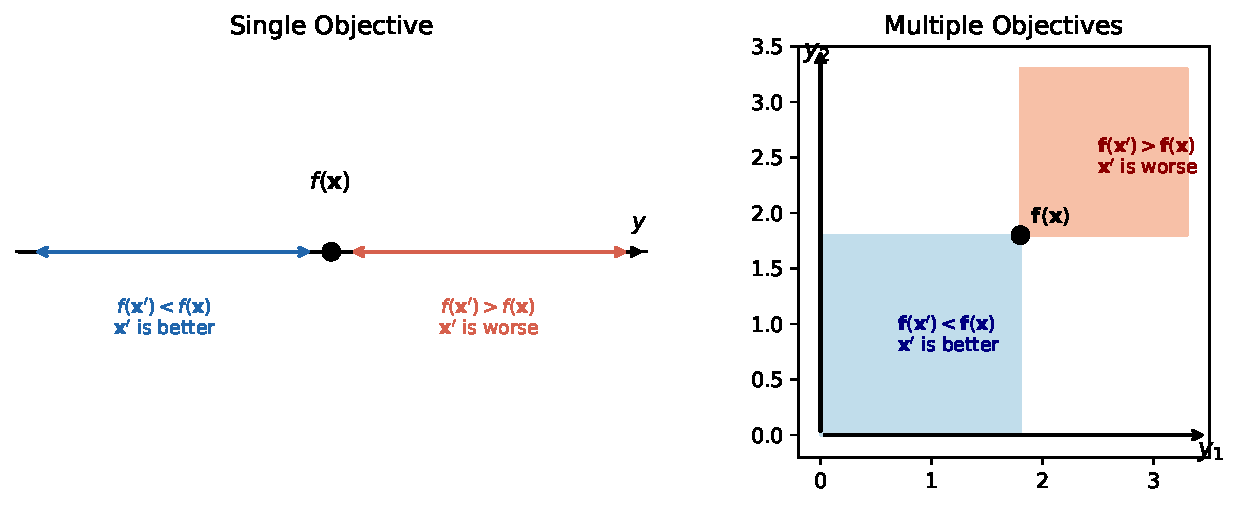
\includegraphics[width=\linewidth]{fig_dominance.pdf}
\end{columns}

\begin{block}{The Ambiguity Region}
  In single-objective optimization, any two solutions are always comparable:
  one must be better or they are equal.  With multiple objectives, however,
  two solutions may be \emph{incomparable}: neither dominates the other.
  This happens when one design is better on some objectives and worse on
  others.  The set of mutually incomparable solutions is where the interesting
  trade-offs live.
\end{block}

\end{frame}

\begin{frame}[fragile]{Dominance in Python}

The \texttt{dominates} function below implements the dominance check using
NumPy's vectorised comparisons.  \texttt{np.all(y <= y\_prime)} returns
\texttt{True} only if \emph{every} element of \texttt{y} is less than or
equal to the corresponding element of \texttt{y\_prime} (condition 1).
\texttt{np.any(y < y\_prime)} returns \texttt{True} if \emph{at least one}
element is strictly smaller (condition 2).  Both must hold for dominance.

\begin{lstlisting}
import numpy as np

def dominates(y: np.ndarray, y_prime: np.ndarray) -> bool:
    """Return True if y dominates y_prime (minimization)."""
    return bool(np.all(y <= y_prime) and np.any(y < y_prime))

# Example: 2 objectives
y  = np.array([1.0, 3.0])
y1 = np.array([2.0, 4.0])  # dominated by y (y is better on BOTH)
y2 = np.array([0.5, 5.0])  # NOT dominated by y (y2 wins on f1)
y3 = np.array([0.5, 2.0])  # dominates y (y3 is better on BOTH)

print(dominates(y, y1))   # True  -- y <= y1 on all, y < y1 on both
print(dominates(y, y2))   # False -- y2[0]=0.5 < y[0]=1.0, so y does NOT win on f1
print(dominates(y3, y))   # True  -- y3 wins on both objectives
\end{lstlisting}

\begin{block}{Key Takeaway}
  The function runs in $O(m)$ time where $m$ is the number of objectives.
  To find all non-dominated points in a set of $n$ designs, we must compare
  every pair, giving $O(n^2 m)$ total work.  A design $\bx$ dominates
  $\bx'$ implies $\bx$ is strictly superior; any two designs with no
  dominance in either direction occupy the ``ambiguity region'' and are
  both potentially worth keeping.
\end{block}

\end{frame}

\begin{frame}[allowframebreaks]{15.1.2 Pareto Frontier}

Once we understand dominance, we can define the central concept of
multiobjective optimization: the Pareto frontier.

\begin{block}{Pareto Optimality}
  A design $\bx \in \mathcal{X}$ is \textbf{Pareto-optimal} if there is no
  other design $\bx' \in \mathcal{X}$ that dominates it.  In other words,
  $\bx$ is Pareto-optimal if it is impossible to improve any one objective
  without worsening at least one other.
\end{block}

\begin{block}{The Pareto Frontier}
  The \textbf{Pareto frontier} (also called the Pareto front or Pareto-optimal
  set) is the collection of \emph{all} Pareto-optimal designs.  In criterion
  space, the Pareto frontier sits on the \emph{lower-left boundary} of
  $\mathcal{Y}$ (for minimization) --- no point in $\mathcal{Y}$ lies further
  to the lower-left.
\end{block}

Every design that is \emph{not} on the Pareto frontier is dominated by at least
one frontier point, meaning it is provably suboptimal and should be discarded.
Only the frontier points represent genuine trade-offs that a rational designer
should consider.

\begin{block}{Weakly Pareto Optimal}
  A design $\bx$ is \textbf{weakly Pareto-optimal} if there is no $\bx'$ such
  that $f_i(\bx') < f_i(\bx)$ for \emph{all} $i$ simultaneously (i.e., no
  design is strictly better on \emph{every} objective).  Every Pareto-optimal
  point is also weakly Pareto-optimal, but the converse is not true: a weakly
  optimal point may be dominated in the regular sense.  The distinction matters
  when choosing algorithms: some methods (e.g., the plain weighted min-max)
  can get stuck at weakly optimal points.
\end{block}

\begin{columns}
\column{0.52\textwidth}
\begin{block}{The Utopia Point (Eq.\ 15.2)}
  The \textbf{utopia point} $\by^{\mathrm{utopia}}$ (sometimes called the
  \emph{ideal} point) is defined component-wise as the individual minimum of
  each objective:
  \[
    y_i^{\mathrm{utopia}} = \min_{\bx \in \mathcal{X}} f_i(\bx),
    \quad i = 1, \ldots, m
  \]
  The subscript $i$ (eye) indexes the objective number.  The utopia point
  answers the question: ``If we cared \emph{only} about objective $i$, what
  is the best we could achieve?''
\end{block}

\begin{alertblock}{How to Read the Utopia Point Formula}
  The formula collects the best possible value for each objective
  \emph{independently}, ignoring all other objectives.  In general, no single
  design achieves all these minima simultaneously --- that is precisely why
  the problem is hard.  The utopia point is therefore usually \emph{not}
  attainable, but it serves as a reference point for measuring how far any
  given design is from the ``dream'' solution.
\end{alertblock}

\column{0.45\textwidth}
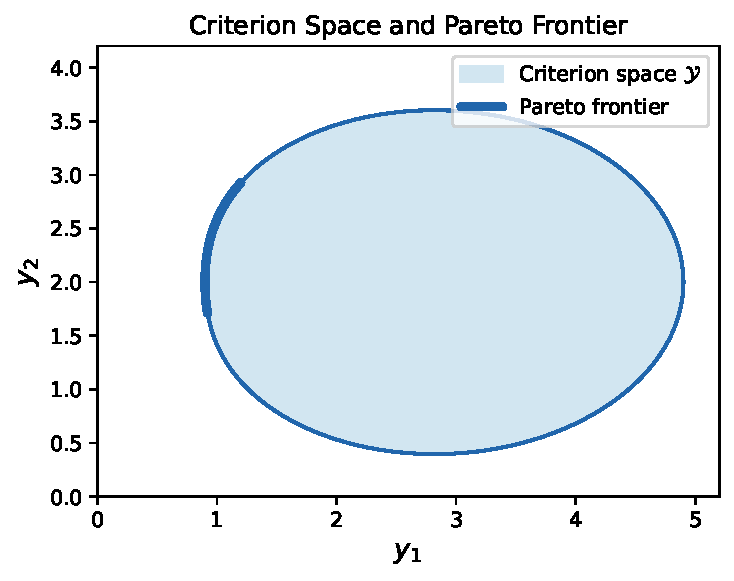
\includegraphics[width=\linewidth]{fig_pareto_frontier.pdf}
\end{columns}

\end{frame}

\begin{frame}[allowframebreaks]{Example 15.1: Aircraft Collision Avoidance}

This example illustrates multiobjective optimization with two competing safety
metrics in an aircraft collision avoidance system.  The system must choose how
aggressively to issue alerts to pilots when aircraft are on potentially
conflicting flight paths.

\begin{columns}
\column{0.52\textwidth}
The two objectives are:
\begin{enumerate}
  \item \textbf{Minimize collision rate $f_1$}: the fraction of near-miss
    encounters that result in an actual collision.  Lower is better.
  \item \textbf{Minimize alert rate $f_2$}: the frequency of alerts issued to
    pilots, including unnecessary ones.  Lower is better.
\end{enumerate}

These objectives are in direct conflict.  Issuing more alerts (increasing
$f_2$) will warn pilots of more potential conflicts, which reduces collisions
(decreasing $f_1$) --- but only if pilots pay attention.  When the alert rate
is very high, pilots become desensitised (``alert fatigue'') and begin ignoring
alerts, which eventually causes collisions to increase again.  A careful
designer must balance these two effects.

\begin{block}{What the Pareto Frontier Tells Us}
  The Pareto frontier for this problem is a curve in the $(f_1, f_2)$ plane.
  Each point on the frontier corresponds to a specific alert policy.  Any
  design whose criterion point lies \emph{above and to the right} of the
  frontier is dominated and therefore suboptimal: a better alert policy exists
  that reduces both collision rate and alert rate simultaneously.  The frontier
  makes clear which trade-offs are achievable and which are not.
\end{block}
\column{0.45\textwidth}
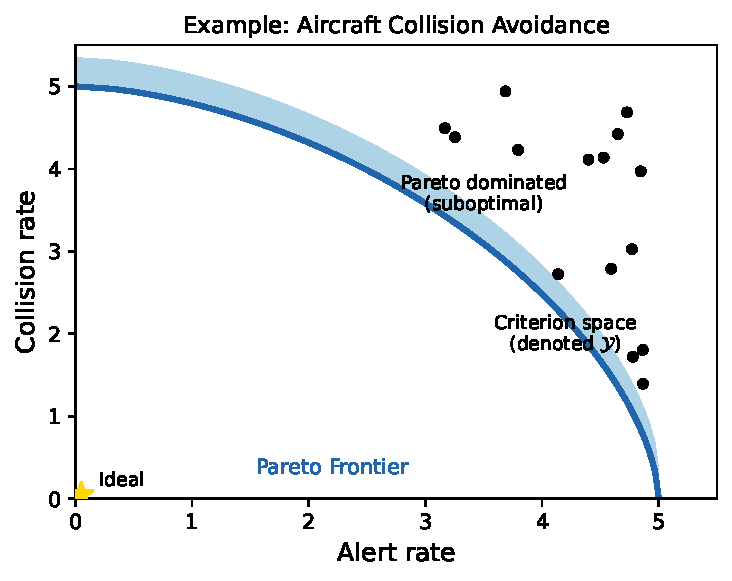
\includegraphics[width=\linewidth]{fig_collision_avoidance.pdf}
\end{columns}

The designer cannot choose ``the best'' point on the frontier without
additional information about how much they value collision reduction relative to
pilot workload.  That preference information is the subject of Section 15.5
(Preference Elicitation).

\end{frame}

\begin{frame}[fragile]{Naive Pareto Filter (Algorithm 15.2)}

Before discussing sophisticated algorithms, it helps to understand the
simplest possible approach to finding the Pareto frontier: check every design
against every other design, and keep only those that are not dominated.  This
is called the \textbf{naive Pareto filter}.

\begin{columns}
\column{0.55\textwidth}
\begin{lstlisting}
import numpy as np

def dominates(y, y_prime):
    return np.all(y <= y_prime) and np.any(y < y_prime)

def naive_pareto(xs, ys):
    """
    xs: list of design points
    ys: list of objective vectors
    Returns (pareto_xs, pareto_ys) -- non-dominated points.
    """
    pareto_xs, pareto_ys = [], []
    for x, y in zip(xs, ys):
        # Keep design x only if NO other point dominates y
        if not any(dominates(yp, y) for yp in ys):
            pareto_xs.append(x)
            pareto_ys.append(y)
    return pareto_xs, pareto_ys

# Example: 200 random designs, 2 objectives
xs = np.random.rand(200, 2)
ys = [np.array([np.linalg.norm(x),
                np.linalg.norm(x - 1)]) for x in xs]
px, py = naive_pareto(xs, ys)
print(f"Pareto points: {len(py)} of {len(ys)}")
\end{lstlisting}

\column{0.42\textwidth}
\begin{block}{Complexity Analysis}
  With $n$ (number of designs) design points and $m$ (number of objectives)
  objectives, the naive filter compares every pair of points and checks all
  $m$ objectives for each comparison.  This gives a total cost of
  $O(n^2 m)$ --- quadratic in the number of designs.  For 200 points and
  2 objectives, that is $200^2 \times 2 = 80{,}000$ comparisons, which is
  fast.  For 10,000 designs and 5 objectives, it becomes $5 \times 10^8$
  comparisons, which is slow.
\end{block}

\begin{alertblock}{Fundamental Limitation}
  Random sampling is extremely inefficient for approximating the Pareto
  frontier.  Most randomly generated points will be dominated and therefore
  discarded.  Structured search methods --- described next --- find better
  trade-off points far more efficiently.
\end{alertblock}
\end{columns}

\end{frame}

% =====================================================================
\section{Constraint Methods}
% =====================================================================

\begin{frame}[allowframebreaks]{15.2.1 The Constraint Method ($\varepsilon$-Constraint)}

The \textbf{constraint method} (also called the $\varepsilon$ (epsilon)
-constraint method) is one of the oldest and most reliable techniques for
tracing the Pareto frontier.  The core idea is simple: instead of trying to
minimize all objectives simultaneously, we designate \emph{one} objective as
the primary objective to minimize, and we turn all remaining objectives into
\emph{inequality constraints} with upper bounds.  By systematically varying
those upper bounds, we move along the Pareto frontier.

\begin{columns}
\column{0.52\textwidth}
\begin{block}{Formulation (Eq.\ 15.3)}
  Minimize $f_1$ subject to upper bounds on all other objectives:
  \[
    \begin{aligned}
      \min_{\bx} &\quad f_1(\bx) \\
      \text{s.t.} &\quad f_2(\bx) \le c_2 \\
                  &\quad \vdots \\
                  &\quad f_m(\bx) \le c_m \\
                  &\quad \bx \in \mathcal{X}
    \end{aligned}
  \]
\end{block}

The symbols $c_2, \ldots, c_m$ (the letter $c$ subscripted by the objective
index) are the constraint bounds.  Setting $c_i$ to a large value effectively
removes the constraint on objective $i$, while setting it to a small value
forces the optimizer to find designs where $f_i$ is small.  The notation
``s.t.'' is shorthand for ``subject to.''

\begin{block}{How to Trace the Frontier}
  We run this optimization repeatedly, each time with a different vector
  $\mathbf{c} = [c_2, \ldots, c_m]^\top$ of constraint bounds.  Each solve
  produces one point on the Pareto frontier.  As $c_i$ decreases from a
  large value (no constraint) down toward the minimum of $f_i$, the optimal
  solution traces out the entire Pareto frontier.
\end{block}

\column{0.45\textwidth}
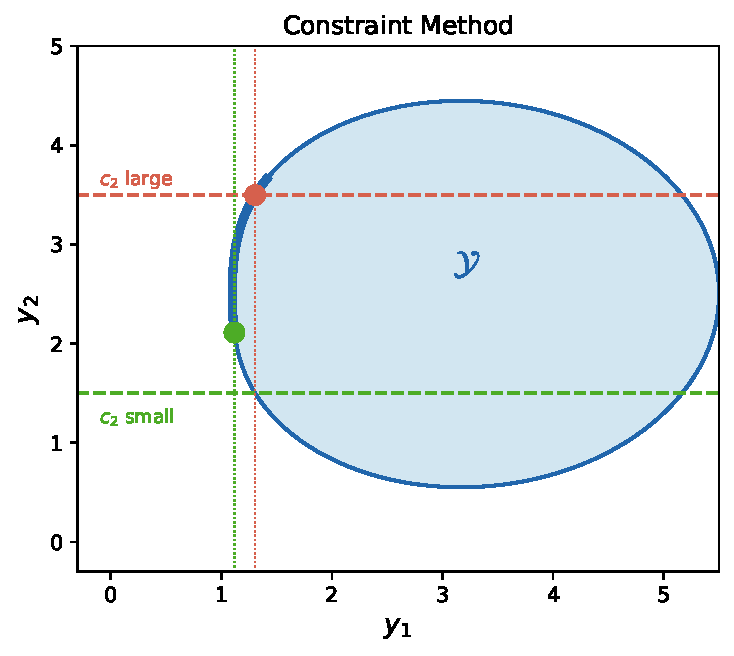
\includegraphics[width=\linewidth]{fig_constraint_method.pdf}
\vspace{0.4em}
\small
As $c_2$ decreases from large to small, the constraint ``pushes'' the optimal
point left along the Pareto frontier, from the extreme that minimises $f_1$
alone to the extreme that minimises $f_2$ alone.
\end{columns}

\begin{alertblock}{Advantage Over Weighted Sum}
  Unlike the weighted sum method (described in Section 15.3), the constraint
  method can find Pareto points in \emph{nonconvex} (concave) regions of the
  frontier.  This is because the constraint boundary can ``probe'' concave
  portions of criterion space, whereas linear weight contours cannot.  The
  constraint method is therefore the more general technique.
\end{alertblock}

\end{frame}

\begin{frame}[fragile]{Constraint Method in Python}

The code below implements the $\varepsilon$-constraint method for two
objectives.  It sweeps a range of values for the constraint $c_2$ (the upper
bound on objective $f_2$) and solves a separate constrained minimisation
for each value, collecting the resulting Pareto points.

\begin{lstlisting}
import numpy as np
from scipy.optimize import minimize

def constraint_method_2d(f1, f2, c2_vals, x0=0.0):
    """
    Sweep c2 values to trace the Pareto frontier (2 objectives).
    f1, f2   : scalar functions of a single variable x
    c2_vals  : array of upper-bound values for f2
    x0       : initial guess for the optimizer
    Returns  : array of (y1, y2) Pareto-optimal pairs
    """
    pareto_pts = []
    for c2 in c2_vals:
        # Constraint: f2(x) <= c2  <=>  c2 - f2(x) >= 0
        result = minimize(
            f1, x0,
            constraints={'type': 'ineq', 'fun': lambda x: c2 - f2(x)},
            method='SLSQP'  # Sequential Least Squares Programming
        )
        if result.success:
            x_opt = result.x[0]
            pareto_pts.append((f1(x_opt), f2(x_opt)))
    return np.array(pareto_pts)

# Exercise 15.7: minimize [x^2, (x-2)^2]
f1 = lambda x: x**2
f2 = lambda x: (x - 2)**2
c2_vals = np.linspace(0.01, 4.0, 50)
front = constraint_method_2d(f1, f2, c2_vals, x0=np.array([1.0]))
\end{lstlisting}

\begin{block}{Result Interpretation}
  The array \texttt{front} contains $(y_1, y_2)$ pairs that trace the Pareto
  curve from $(0, 4)$ (where $x=0$, achieving $f_1=0$ but $f_2=(0-2)^2=4$) to
  $(4, 0)$ (where $x=2$, achieving $f_2=0$ but $f_1=4$).  Each row is one
  Pareto-optimal design, obtainable at no cost to any other objective.
\end{block}

\end{frame}

\begin{frame}[allowframebreaks]{15.2.2 Lexicographic Method}

The \textbf{lexicographic method} addresses multiobjective problems when the
designer can specify a strict \emph{priority ordering} among objectives ---
that is, when objective 1 matters more than objective 2, which matters more
than objective 3, and so on.  The name ``lexicographic'' comes from the
dictionary: in a dictionary, words are sorted first by their first letter,
then (for ties) by their second letter, and so on.

\begin{columns}
\column{0.55\textwidth}
\begin{block}{Procedure}
  Rank all $m$ objectives from most important ($f_1$) to least important
  ($f_m$).  Then solve $m$ optimisation problems sequentially, adding one
  constraint at each step:
  \begin{enumerate}
    \item Minimize $f_1$ over $\mathcal{X}$.  Let the optimal value be
      $y_1^* = \min f_1$.
    \item Minimize $f_2$ subject to $f_1(\bx) \le y_1^*$ (do not allow
      $f_1$ to worsen).  Let $y_2^* = \min f_2$ under this constraint.
    \item Minimize $f_3$ subject to $f_1(\bx) \le y_1^*$ and
      $f_2(\bx) \le y_2^*$.  Let $y_3^* = \min f_3$.
    \item Continue in this manner through objective $m$.
  \end{enumerate}
  Each step preserves all previously attained optimal values.
\end{block}

\begin{itemize}
  \item The method is always feasible: since $y_k^*$ was achieved in step $k$,
    the feasible set at step $k+1$ is non-empty (the solution from step $k$
    is always available).

  \item The method produces a \textbf{single} Pareto-optimal point --- the one
    that best satisfies objectives in priority order.  It does not produce the
    full frontier.

  \item Using inequality constraints $f_k(\bx) \le y_k^*$ (rather than
    equalities $f_k(\bx) = y_k^*$) is preferred in practice: if the solver is
    slightly suboptimal in an early step, the inequality constraint is still
    satisfiable, whereas an equality constraint might not be.
\end{itemize}

\column{0.42\textwidth}
\begin{alertblock}{Critical Limitation}
  The lexicographic method yields only \emph{one} design point, not the full
  Pareto frontier.  Furthermore, the result is highly sensitive to the
  priority ordering: different rankings of objectives will generally produce
  different final designs, and there is no systematic way to recover other
  Pareto-optimal designs without re-running the entire procedure with a
  different ordering.
\end{alertblock}

\begin{exampleblock}{Ideal Use Case}
  Use the lexicographic method when there is a genuine, well-justified
  priority ranking among objectives --- for instance, in a safety-critical
  system where ``no fatalities'' (objective 1) always trumps ``minimise cost''
  (objective 2), which always trumps ``minimise weight'' (objective 3).  In
  such settings, the strict priority ordering is ethically and practically
  meaningful.
\end{exampleblock}
\end{columns}

\end{frame}

% =====================================================================
\section{Weight Methods}
% =====================================================================

\begin{frame}[allowframebreaks]{15.3.1 Weighted Sum Method}

The \textbf{weighted sum method} is the most intuitive scalarisation approach:
we assign a non-negative weight $w_i$ (w sub $i$) to each objective $f_i$,
then minimise the weighted total.  Intuitively, each weight represents how
much we ``care about'' the corresponding objective relative to the others.

\begin{columns}
\column{0.52\textwidth}
\begin{block}{Weighted Sum Objective (Eq.\ 15.4)}
  \[
    f(\bx) = \bw^\top \bff(\bx) = \sum_{i=1}^{m} w_i f_i(\bx)
  \]
  subject to $w_i \ge 0$ for all $i$ (no negative weights) and
  $\sum_{i=1}^m w_i = 1$ (weights sum to one, forming a probability simplex).
\end{block}

Here $\bw = [w_1, w_2, \ldots, w_m]^\top$ (bold $w$) is the weight vector.
The notation $\bw^\top \bff(\bx)$ is the \emph{dot product} (or inner
product) of $\bw$ and $\bff(\bx)$, which equals
$\sum_{i=1}^m w_i f_i(\bx)$ --- the sum (written with $\sum$, Sigma,
meaning ``add up all the following terms'') of each weight multiplied by the
corresponding objective.  The index $i$ runs from $1$ to $m$.

\begin{alertblock}{How to Read This Formula}
  Imagine each objective $f_i(\bx)$ has a price tag $w_i$.  The weighted sum
  $f(\bx)$ is the total ``cost'' of design $\bx$.  A large $w_1$ means
  objective 1 dominates the total, so the optimizer will prioritise minimising
  $f_1$.  Setting $w_1 = 1, w_2 = 0$ recovers pure single-objective
  optimisation on $f_1$ alone.  By sweeping $\bw$ across the unit simplex
  (all non-negative weight vectors summing to 1), we trace out different
  Pareto-optimal points.
\end{alertblock}

\column{0.45\textwidth}
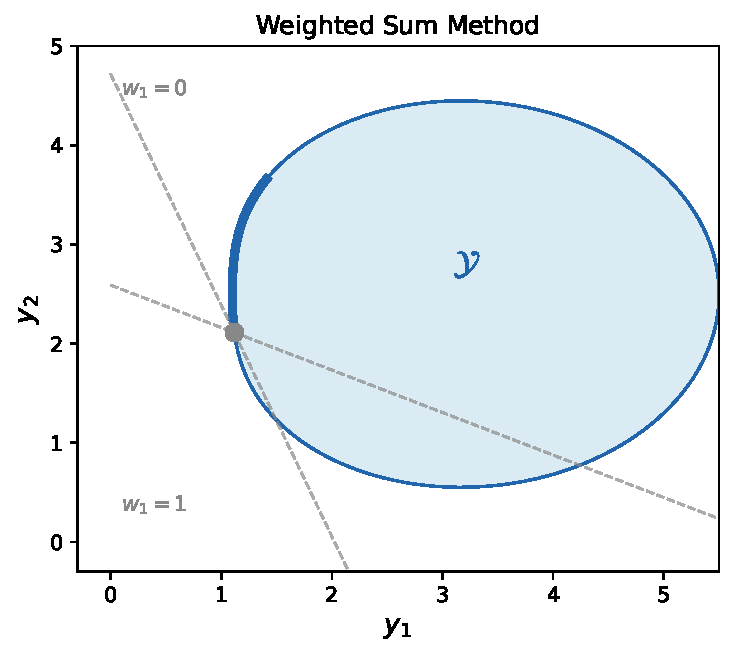
\includegraphics[width=\linewidth]{fig_weighted_sum.pdf}
\end{columns}

\begin{block}{Tracing the Frontier in 2D}
  With two objectives ($m=2$), the weight simplex is just the interval
  $[0, 1]$: set $w_1 \in [0, 1]$ and $w_2 = 1 - w_1$.  As $w_1$ increases
  from 0 to 1, the optimizer shifts from minimising $f_2$ alone to minimising
  $f_1$ alone, sweeping through different trade-off points.
\end{block}

\begin{alertblock}{Critical Limitation: Nonconvex Frontiers}
  The weighted sum method \textbf{cannot} find Pareto-optimal points in
  \emph{nonconvex} regions of the frontier.  Geometrically, the iso-cost
  lines of the weighted sum are \emph{hyperplanes} (straight lines in 2D).
  When the Pareto frontier is concave (bends inward), no hyperplane can be
  tangent to it, so the optimizer jumps over the concave portion entirely.
  For nonconvex frontiers, use the constraint method (Section 15.2) or
  the min-max method (Section 15.3.3) instead.
\end{alertblock}

\end{frame}

\begin{frame}[fragile]{Weighted Sum in Python}

\begin{lstlisting}
import numpy as np
from scipy.optimize import minimize

def weight_pareto(f1, f2, n_pts=50, x0=0.0):
    """
    Weighted sum method: sweep w1 from 0 to 1 in n_pts steps.
    Returns array of (y1, y2) Pareto-optimal points.
    """
    results = []
    for w1 in np.linspace(0, 1, n_pts):
        w2 = 1.0 - w1
        # Combined objective: w1*f1(x) + w2*f2(x)
        obj = lambda x: w1 * f1(x) + w2 * f2(x)
        res = minimize(obj, x0, method='BFGS')
        if res.success:
            x_opt = res.x[0]
            results.append((f1(x_opt), f2(x_opt)))
    return np.array(results)

# Example: f1(x) = x^2, f2(x) = (x-2)^2
f1 = lambda x: float(x**2)
f2 = lambda x: float((x - 2)**2)
front = weight_pareto(f1, f2, n_pts=30, x0=np.array([1.0]))
# Note: For these convex functions, weighted sum works correctly.
# On nonconvex frontiers, it would skip concave portions!
\end{lstlisting}

\begin{exampleblock}{Worked Numerical Example (3 Weight Choices)}
  With $f_1(x) = x^2$ and $f_2(x) = (x-2)^2$, the combined objective is
  $w_1 x^2 + w_2 (x-2)^2$.  Taking the derivative and setting to zero:
  $2 w_1 x + 2 w_2 (x-2) = 0$, giving $x^* = 2w_2 / (w_1 + w_2) = 2w_2$
  (since $w_1 + w_2 = 1$).

  \begin{center}
  \begin{tabular}{lccc}
  \toprule
  $w_1$ & $x^*$ & $f_1 = (x^*)^2$ & $f_2 = (x^*-2)^2$ \\
  \midrule
  0.1 & $2 \times 0.9 = 1.8$ & $1.8^2 = 3.24$ & $(1.8-2)^2 = 0.04$ \\
  0.5 & $2 \times 0.5 = 1.0$ & $1.0^2 = 1.00$ & $(1.0-2)^2 = 1.00$ \\
  0.9 & $2 \times 0.1 = 0.2$ & $0.2^2 = 0.04$ & $(0.2-2)^2 = 3.24$ \\
  \bottomrule
  \end{tabular}
  \end{center}
  As $w_1$ increases, the optimizer drives $x^*$ toward 0 (minimising $f_1$)
  and away from 2 (allowing $f_2$ to grow).
\end{exampleblock}

\end{frame}

\begin{frame}[allowframebreaks]{15.3.2 Goal Programming}

\textbf{Goal programming} addresses a natural question: ``We know the utopia
point (the best we could achieve on each objective independently) --- how do
we find designs that are \emph{as close as possible} to this ideal?''  The
idea is to minimise the distance between the current objective vector and the
desired \emph{goal point}.

\begin{columns}
\column{0.55\textwidth}
\begin{block}{$L_p$ Goal Programming (Eq.\ 15.5)}
  Minimise the $L_p$ (L-p, read ``L-$p$-norm'') distance from the objective
  vector $\bff(\bx)$ to the goal point $\by^{\mathrm{goal}}$:
  \[
    \min_{\bx \in \mathcal{X}}\;
    \left\|\bff(\bx) - \by^{\mathrm{goal}}\right\|_p
  \]
  The goal point is typically set to the \textbf{utopia point}: the
  best achievable values for each objective independently.
\end{block}

Here $\|\cdot\|_p$ (norm with subscript $p$, where $p \ge 1$ is a positive
real number) measures ``distance'' in a generalised sense.  The formula
$\|\bff(\bx) - \by^{\mathrm{goal}}\|_p$ computes how far the achieved
objective vector is from the goal.  Different choices of $p$ give different
shapes of ``distance ball,'' which in turn determine which Pareto-optimal
point is found.

\begin{block}{Weighted Exponential Sum (Eq.\ 15.6)}
  A weighted generalisation:
  \[
    f(\bx) = \sum_{i=1}^{m} w_i
    \left|f_i(\bx) - y_i^{\mathrm{goal}}\right|^p
  \]
  Here $w_i \ge 0$ with $\sum_i w_i = 1$ are weights, $p \ge 1$ is the
  exponent, $y_i^{\mathrm{goal}}$ (y sub $i$ superscript goal) is the
  $i$-th component of the goal vector, and $|\cdot|$ denotes absolute value.
  The symbol $\sum$ (Sigma) means ``sum over all $i$ from 1 to $m$.''
\end{block}

\column{0.42\textwidth}
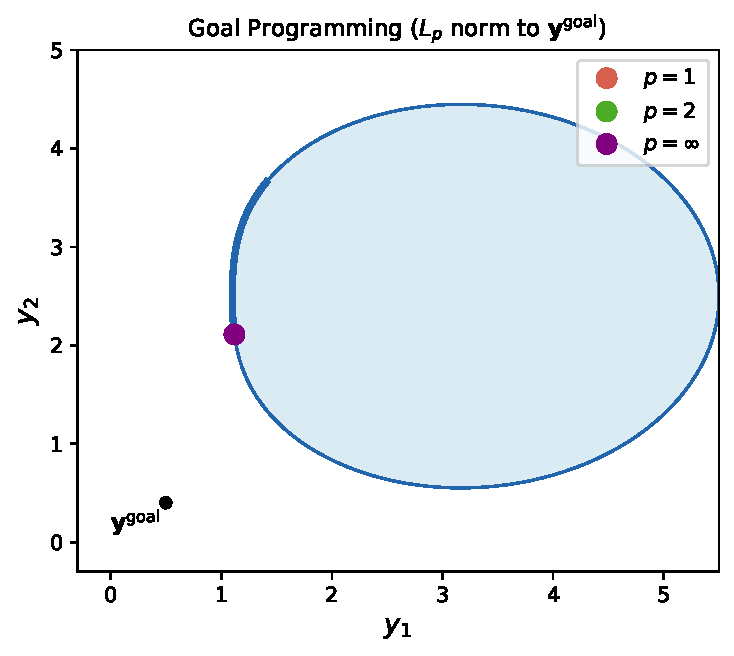
\includegraphics[width=\linewidth]{fig_goal_programming.pdf}
\vspace{0.3em}
\small Different values of $p$ change the shape of the iso-cost contours and
therefore reach different Pareto-optimal points.
\end{columns}

\begin{block}{Effect of Different $p$ Values}
  \begin{itemize}
    \item $p = 1$ gives the \textbf{Manhattan distance} (L1 norm): the sum of
      absolute differences in each objective.  The contours are diamond-shaped.

    \item $p = 2$ gives the standard \textbf{Euclidean distance}: the
      straight-line distance to the goal.  The contours are circles (in 2D) or
      spheres (in higher dimensions).

    \item $p \to \infty$ gives the \textbf{Chebyshev distance} (also called
      min-max): the distance equals the largest single-objective deviation.
      The contours are squares.  This is the subject of Section 15.3.3.
  \end{itemize}
  As $p$ increases, the norm pays increasing attention to the \emph{worst}
  (largest) objective deviation, eventually focusing entirely on it.
\end{block}

\end{frame}

\begin{frame}[allowframebreaks]{15.3.3--15.3.5 Advanced Weight Methods}

This section covers three important generalisations beyond the simple weighted
sum: the weighted min-max method (Tchebycheff approach), its augmented version,
and the exponential weighted criterion.  All three can recover Pareto-optimal
points in nonconvex frontier regions that the weighted sum misses.

\begin{columns}
\column{0.5\textwidth}
\begin{block}{Weighted Min-Max / Tchebycheff (Eq.\ 15.7)}
  Instead of summing weighted objectives, take the \emph{maximum}:
  \[
    f(\bx) = \max_{i \in \{1,\ldots,m\}}
    \left[ w_i \left( f_i(\bx) - y_i^{\mathrm{goal}} \right) \right]
  \]
  Here $\max$ selects the largest value across all $i$.  The term
  $f_i(\bx) - y_i^{\mathrm{goal}}$ (f sub $i$ minus y sub $i$ superscript
  goal) measures how far objective $i$ is above the goal; multiplying by
  $w_i$ (w sub $i$) scales it by the objective's importance.
\end{block}

\begin{alertblock}{How to Read This Formula}
  The formula finds the \emph{most violated} (furthest above goal) weighted
  objective and returns that value.  Minimising this quantity means minimising
  the worst-case weighted deviation --- we try to ensure no objective is too
  far above its goal.  Geometrically, the iso-cost contours are
  \emph{diamond-shaped} (in 2D), which allows them to ``reach into'' concave
  portions of the Pareto frontier where linear contours cannot enter.
\end{alertblock}

\begin{itemize}
  \item This method is the limit of the weighted exponential sum
    (Eq.~15.6) as $p \to \infty$.
  \item By varying $\bw$ across the weight simplex, one can recover
    the \textbf{complete} Pareto-optimal set --- including points in
    nonconvex frontier regions.
  \item However, in its basic form, it may also produce
    \emph{weakly} Pareto-optimal points (not strictly optimal).
\end{itemize}

\column{0.47\textwidth}
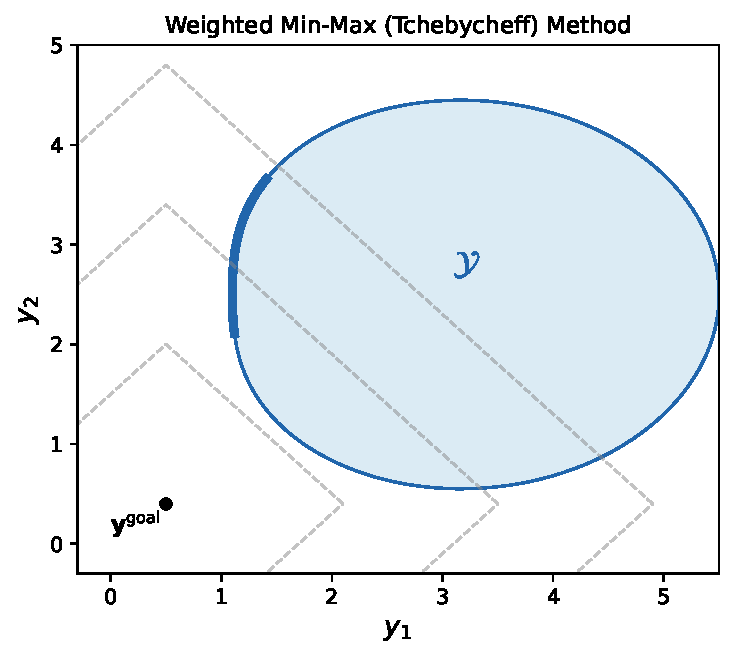
\includegraphics[width=\linewidth]{fig_weighted_minmax.pdf}

\begin{block}{Augmented Tchebycheff (Eq.\ 15.8)}
  Adding a small regularisation term to the min-max objective:
  \[
    f(\bx) = \max_i\!\left[w_i\!\left(f_i(\bx) - y_i^{\mathrm{goal}}\right)\right]
    + \rho\,\bff(\bx)^\top \by^{\mathrm{goal}}
  \]
  Here $\rho$ (rho, a small Greek letter) is a tiny positive scalar,
  typically $\rho \in (0.0001,\; 0.01)$.  The term
  $\bff(\bx)^\top \by^{\mathrm{goal}}$ is the dot product of the objective
  vector with the goal vector.  This small perturbation eliminates
  weakly Pareto-optimal solutions, ensuring all found points are
  \emph{strictly} Pareto-optimal.
\end{block}
\end{columns}

\begin{block}{Exponential Weighted Criterion (Eq.\ 15.9)}
  A different approach to handle nonconvex frontiers:
  \[
    f(\bx) = \sum_{i=1}^{m} \left(e^{p w_i} - 1\right) e^{p f_i(\bx)}
  \]
  Here $e$ is Euler's number ($e \approx 2.718$), $p$ (the letter $p$) is
  a positive scaling parameter, and $e^x$ (e to the power $x$) is the
  exponential function.  The term $(e^{p w_i} - 1)$ depends on the weight
  $w_i$ and scales nonlinearly with $p$.  Unlike the weighted sum, this
  criterion produces nonlinear contours that can reach nonconvex regions.
  However, large values of $p$ can cause numerical overflow in the
  exponential terms, so care is needed.
\end{block}

\end{frame}

\begin{frame}[fragile]{Weighted Min-Max in Python}

The code below implements the \textbf{augmented Tchebycheff} method.  The
small perturbation parameter \texttt{rho} ($\rho$, rho) is set to $10^{-3}$
by default, which is well within the recommended range of $0.0001$ to $0.01$.

\begin{lstlisting}
import numpy as np
from scipy.optimize import minimize

def weighted_minmax(f_list, w, y_goal, x0, rho=1e-3):
    """
    Augmented Tchebycheff (weighted min-max + small perturbation).
    f_list : list of objective functions [f1, f2, ...]
    w      : weight vector (non-negative, sums to 1)
    y_goal : goal/utopia point (target for each objective)
    rho    : small scalar in (0.0001, 0.01); default 0.001
    x0     : initial guess for optimizer
    """
    def objective(x):
        ys = np.array([fi(x) for fi in f_list])
        # Tchebycheff term: maximum weighted deviation from goal
        cheby = np.max(w * (ys - y_goal))
        # Augmentation: small dot-product perturbation
        return cheby + rho * np.dot(ys, y_goal)

    res = minimize(objective, x0, method='Nelder-Mead')
    return res

# Example: 2 objectives on R^2
f1 = lambda x: x[0]**2 + x[1]**2
f2 = lambda x: (x[0]-2)**2 + (x[1]-1)**2
w  = np.array([0.5, 0.5])
yg = np.array([0.0, 0.0])   # approximate utopia point
res = weighted_minmax([f1, f2], w, yg, x0=np.array([1.0, 1.0]))
print("Optimal x:", res.x)
print("Objectives:", f1(res.x), f2(res.x))
\end{lstlisting}

\begin{exampleblock}{Interpreting the Output}
  With equal weights $w_1 = w_2 = 0.5$ and the utopia point at the origin,
  the Tchebycheff objective penalises whichever of $f_1(\bx)$ or
  $f_2(\bx)$ is larger.  The optimizer finds the point where both objectives
  are approximately equal, which corresponds to the ``balanced'' point on the
  Pareto frontier.  Varying the weights shifts this balance point toward
  either extreme of the frontier.
\end{exampleblock}

\end{frame}

\begin{frame}[allowframebreaks]{Comparison of Weight Methods}

The table below summarises when each scalarisation method can and cannot
find Pareto-optimal points.  The column ``Nonconvex frontier?'' is the most
important distinguisher: if the Pareto frontier has concave (inward-curving)
sections, the weighted sum method will miss them entirely.

\begin{center}
\begin{tabular}{lcccc}
\toprule
\textbf{Method} & \textbf{Convex frontier?} & \textbf{Nonconvex frontier?} & \textbf{Full coverage} & \textbf{Complexity} \\
\midrule
Weighted Sum         & Yes & No         & Partial & $O(n_w \cdot T_{\text{opt}})$ \\
Goal Programming     & Yes & Partial    & No      & $O(n_p \cdot T_{\text{opt}})$ \\
Wtd.\ Exp.\ Sum     & Yes & Yes        & Partial & $O(n_w \cdot T_{\text{opt}})$ \\
Wtd.\ Min-Max        & Yes & Yes        & Yes*    & $O(n_w \cdot T_{\text{opt}})$ \\
Constraint Method    & Yes & Yes        & Yes     & $O(n_c \cdot T_{\text{opt}})$ \\
\bottomrule
\end{tabular}
\end{center}

The symbols in the complexity column mean: $n_w$ is the number of weight
vectors tried, $n_p$ is the number of exponent values tried, $n_c$ is the
number of constraint levels swept, and $T_{\text{opt}}$ is the cost of
solving one single-objective optimization problem (the ``inner'' problem for
each parameter setting).

\textbf{Note on ``Full coverage'':}  ``Yes*'' for Weighted Min-Max means the
\emph{augmented} form (Eq.~15.8, with the $\rho$ term) achieves full coverage;
the plain form may produce weakly Pareto-optimal points.  The constraint method
achieves complete coverage in theory, though in practice a finite grid of
$c$ values covers the frontier only approximately.

\begin{alertblock}{Practical Recommendation}
  For problems where the Pareto frontier is known to be convex (e.g., convex
  objectives with convex constraints), the weighted sum method is simplest and
  sufficient.  For general problems, use the augmented Tchebycheff (weighted
  min-max) method or the constraint method.  The constraint method is
  particularly reliable for nonconvex frontiers because it does not rely on
  the geometric shape of iso-cost contours.
\end{alertblock}

\end{frame}

% =====================================================================
\section{Multiobjective Population Methods}
% =====================================================================

\begin{frame}[allowframebreaks]{15.4 Multiobjective Population Methods: Overview}

All the methods in Sections 15.2 and 15.3 are \emph{scalarisation} approaches:
they convert the multiobjective problem into a sequence of single-objective
problems, each solved independently.  To obtain $k$ Pareto-optimal points,
they require $k$ separate optimisation runs.

\textbf{Population methods} take a fundamentally different approach.  They
maintain a \emph{population} (a collection) of many candidate designs and
evolve all of them simultaneously.  Because the population explores many
regions of the design space at once, a single run can discover a diverse
collection of Pareto-optimal points --- one for each ``niche'' along the
frontier.

\begin{columns}
\column{0.55\textwidth}
\begin{block}{Four Main Approaches}
  \begin{enumerate}
    \item \textbf{Subpopulations} (Section 15.4.1): divide the population into
      $m$ groups, each optimising a different objective.  Cross-breeding
      between groups explores the trade-off space.

    \item \textbf{Nondomination ranking} (Section 15.4.2): assign each
      individual a rank based on how many ``layers'' of dominance separate it
      from the current Pareto front.  Lower rank is better.  This is the
      basis of NSGA-II.

    \item \textbf{Pareto filters} (Section 15.4.3): maintain a separate
      ``elite archive'' of the best (non-dominated) individuals found so far,
      updated incrementally as the population evolves.

    \item \textbf{Niche techniques} (Section 15.4.4): add mechanisms to
      \emph{spread} the population across the frontier, preventing it from
      clustering in one region.
  \end{enumerate}
\end{block}

\column{0.42\textwidth}
\begin{exampleblock}{Why Population Methods Excel}
  A single run produces \emph{many} Pareto-optimal points, not just one.
  No scalarisation is required --- the method operates directly in the
  criterion space.  Population methods handle nonconvex, disconnected, and
  non-smooth frontiers naturally.  Their built-in diversity mechanisms
  promote spread across the entire frontier.
\end{exampleblock}
\end{columns}

\end{frame}

\begin{frame}[allowframebreaks]{15.4.1 Vector Evaluated Genetic Algorithm (Algorithm 15.4)}

The \textbf{Vector Evaluated Genetic Algorithm} (VEGA) is the earliest
population-based multiobjective method.  Its key insight is that a
single population can be split into specialised subgroups, each focusing on
one objective, while cross-breeding between subgroups maintains information
about all objectives simultaneously.

\begin{columns}
\column{0.55\textwidth}
\begin{block}{VEGA Algorithm}
  Given a population of $n_{\text{pop}}$ individuals and $m$ objectives:
  \begin{enumerate}
    \item \textbf{Evaluate}: compute $\by_i = \bff(\bx_i)$ for every
      individual $\bx_i$ in the population.  Here $\by_i$ (bold $y$ sub $i$)
      is the objective vector for individual $i$.

    \item \textbf{Partition}: split the population into $m$ subpopulations of
      equal size $n_{\text{pop}} / m$.

    \item \textbf{Select}: subpopulation $k$ selects parents by fitness on
      objective $f_k$ \emph{only}, ignoring all other objectives.  This
      allows each subgroup to specialise.

    \item \textbf{Shuffle}: randomly permute all selected parents across
      the $m$ subpopulations.  This mixes genetic material between
      specialists.

    \item \textbf{Breed}: apply crossover (recombination) and mutation to
      the shuffled parents to form the next generation.
  \end{enumerate}
\end{block}

\begin{itemize}
  \item Crossover between subpopulations prevents over-specialisation and
    maintains genetic diversity.
  \item VEGA tends to converge to the \emph{extreme} points of the Pareto
    frontier (the endpoints), missing the middle portions.
\end{itemize}

\column{0.42\textwidth}
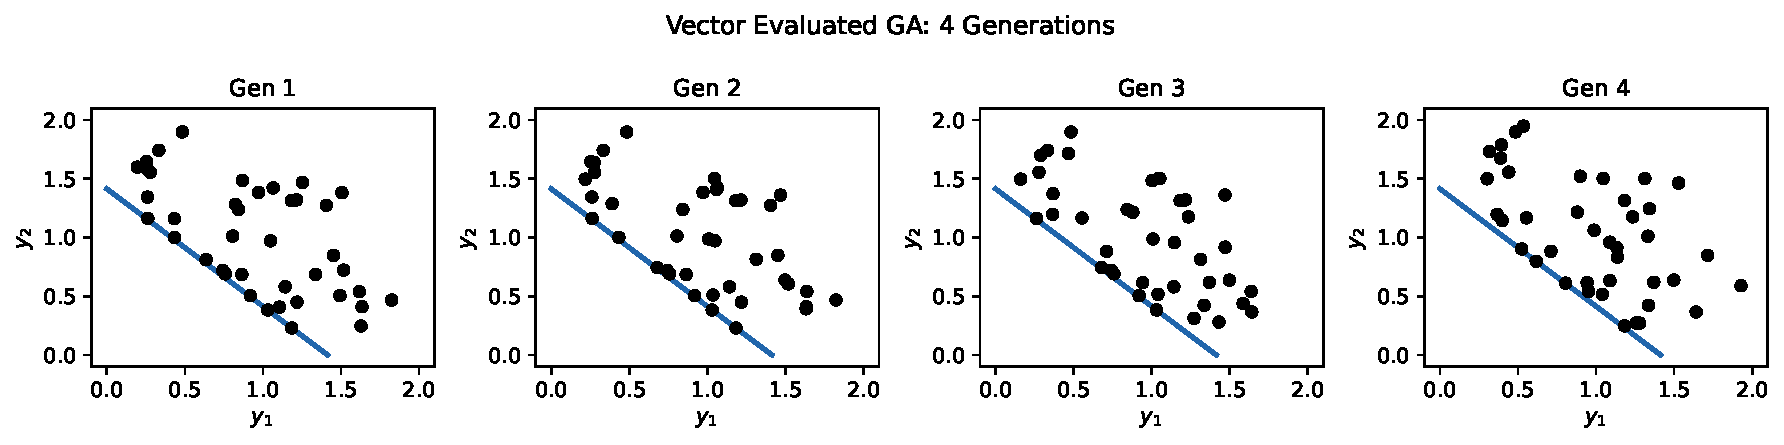
\includegraphics[width=\linewidth]{fig_nsga_evolution.pdf}
\small The population (coloured circles) evolves toward the Pareto frontier
(solid curve) over successive generations.  Early generations are scattered;
later generations cluster near the frontier.
\end{columns}

\begin{alertblock}{Key Insight}
  VEGA's shuffling step is what makes it work: by mixing parents selected
  under different objectives, offspring inherit traits that are good for
  \emph{multiple} objectives simultaneously.  Without shuffling, each
  subpopulation would evolve independently and the method would degenerate
  into $m$ separate single-objective optimisers.
\end{alertblock}

\end{frame}

\begin{frame}[fragile]{VEGA in Python}

The code below implements one generation of VEGA.  The helper
\texttt{tournament\_select} function uses tournament selection: pick two
individuals at random, and return the one with the better (lower) fitness.
This probabilistically favours better individuals without completely
eliminating worse ones, maintaining diversity.

\begin{lstlisting}
import numpy as np

def tournament_select(fitness, n_select):
    """Simple tournament selection: pick 2 at random, keep the better."""
    # fitness: array of scalar fitness values (lower is better)
    # n_select: how many winners to return
    idx = np.random.choice(len(fitness), size=(n_select, 2))
    # argmin along axis=1: pick the index with lower fitness in each pair
    winners = idx[range(n_select),
                  np.argmin(fitness[idx], axis=1)]
    return winners

def vega_step(population, f_list):
    """
    One generation of VEGA.
    population : (n_pop, d) array of design vectors
    f_list     : list of m objective functions
    Returns    : new population of same size
    """
    m = len(f_list)
    n_pop = len(population)
    n_sub = n_pop // m   # size of each subpopulation

    # Step 1: Evaluate all objectives for every individual
    ys = np.array([[fi(x) for fi in f_list] for x in population])

    # Steps 2-3: Each subpopulation selects parents by its own objective
    parents = []
    for k in range(m):
        fitness_k = ys[:, k]  # objective k for all individuals
        sel = tournament_select(fitness_k, n_sub)
        parents.extend(sel.tolist())

    # Step 4: Shuffle parents to mix subpopulations
    parents = np.random.permutation(parents)

    # Step 5: Crossover + mutation
    new_pop = []
    for i in range(0, n_pop, 2):
        p1, p2 = population[parents[i]], population[parents[i+1]]
        alpha = np.random.rand(*p1.shape)   # random blend coefficient
        child = alpha * p1 + (1 - alpha) * p2   # convex combination
        child += 0.05 * np.random.randn(*child.shape)  # Gaussian mutation
        new_pop.append(child)
    return np.array(new_pop)
\end{lstlisting}

\end{frame}

\begin{frame}[allowframebreaks]{15.4.2 Nondomination Ranking (Algorithm 15.5)}

\textbf{Nondomination ranking} is the key innovation in
\textbf{NSGA-II} (Non-dominated Sorting Genetic Algorithm, version 2),
which is currently the most widely used multiobjective evolutionary
algorithm.  The idea is to assign every individual in the population a
\emph{rank} (level) that measures how ``deep'' it is inside the dominated
region.

\begin{columns}
\column{0.52\textwidth}
\begin{block}{NSGA-II Ranking Levels}
  \begin{description}
    \item[Level 1:] The set of individuals that are not dominated by any
      other individual in the \emph{entire} population.  These are the
      current best approximation to the Pareto frontier.
    \item[Level 2:] The non-dominated individuals in the population after
      all Level 1 individuals are removed.  These are the next-best designs.
    \item[Level $k$ (k-th level):] The non-dominated individuals
      after removing Levels 1 through $k-1$.  Each successive level is
      dominated by the previous levels.
  \end{description}
  The process continues until every individual has been assigned a level.
\end{block}

\begin{block}{Selection Rule}
  During evolution, Level 1 individuals are preferred over Level 2, Level 2
  over Level 3, and so on.  When two individuals have the \emph{same} level
  (i.e., they are mutually non-dominated relative to each other and to the
  rest), a tiebreaker called \textbf{crowding distance} is used: prefer the
  individual that has fewer neighbours nearby in criterion space, thereby
  maintaining diversity along the frontier.
\end{block}

\begin{itemize}
  \item Reference: Deb et al., ``A fast and elitist multiobjective genetic
    algorithm: NSGA-II,'' \emph{IEEE Transactions on Evolutionary
    Computation}, 2002.
\end{itemize}

\column{0.45\textwidth}
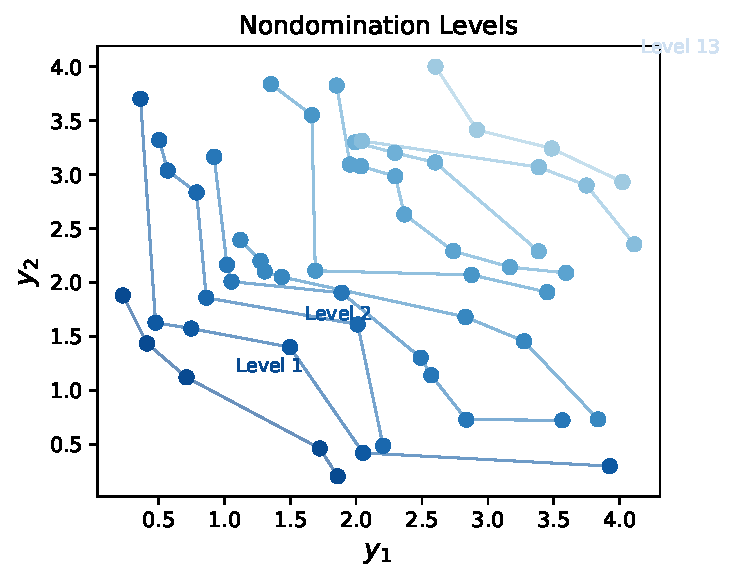
\includegraphics[width=\linewidth]{fig_nondomination_levels.pdf}
\small Darker shading indicates a lower (better) nondomination level.
Level 1 points (darkest) are the current Pareto frontier approximation;
higher levels (lighter) are progressively more dominated.
\end{columns}

\begin{alertblock}{Key Advantage of NSGA-II}
  By explicitly maintaining multiple nondomination levels, NSGA-II ensures
  that the best individuals (Level 1) are always preserved across generations
  (elitism), while still exploring new regions through crossover and mutation.
  The crowding distance tiebreaker prevents the population from collapsing
  to a small cluster, ensuring a well-distributed approximation of the full
  Pareto frontier.
\end{alertblock}

\end{frame}

\begin{frame}[fragile]{Nondomination Ranking in Python}

The function below assigns a nondomination level to each objective vector
in a set.  It works by iteratively extracting the non-dominated front: at
each iteration, all currently ``unranked'' (assigned level 0) points are
checked, and those not dominated by any other unranked point are assigned
the current level.  This process repeats until all points are ranked.

\begin{lstlisting}
import numpy as np

def dominates(y, y_prime):
    """True if y dominates y_prime (y is at least as good on all, better on some)."""
    return np.all(y <= y_prime) and np.any(y < y_prime)

def nondomination_levels(ys):
    """
    Assign nondomination levels to a set of objective vectors.
    Level 1 = non-dominated in full set (best).
    Level 2 = non-dominated after removing Level 1.
    ...and so on.
    ys     : (n, m) array of objective values
    Returns: levels array of shape (n,), with values 1, 2, 3, ...
    """
    n = len(ys)
    levels = np.zeros(n, dtype=int)  # 0 = not yet assigned
    L = 0
    while np.any(levels == 0):       # while some points unranked
        L += 1
        for i in range(n):
            if levels[i] == 0:       # only consider unranked points
                dominated = False
                for j in range(n):
                    if j != i and (levels[j] == 0 or levels[j] == L):
                        if dominates(ys[j], ys[i]):
                            dominated = True
                            break
                if not dominated:
                    levels[i] = L    # assign current level
    return levels

# Usage example:
ys = np.array([[1, 3], [2, 2], [3, 1], [2, 3], [1.5, 2.5]])
print(nondomination_levels(ys))
# Expected: [1,3],[2,2],[3,1] are Level 1; [2,3],[1.5,2.5] are Level 2
\end{lstlisting}

\end{frame}

\begin{frame}[allowframebreaks]{15.4.3 Pareto Filters (Algorithm 15.7)}

A \textbf{Pareto filter} (also called an \emph{elite archive}) is a data
structure that maintains a compact, up-to-date set of the best
(non-dominated) designs found by a population method.  As the population
evolves, new individuals are evaluated and the filter is updated: dominated
points are removed and newly non-dominated points are added.  When the
filter reaches its maximum capacity, a pruning rule removes one point from
the closest pair to maintain diversity.

\begin{columns}
\column{0.52\textwidth}
\begin{block}{Pareto Filter Update Procedure}
  Given a new individual $(x, \by)$ where $\by = \bff(x)$:
  \begin{enumerate}
    \item If $\by$ is dominated by any point $\by'$ already in the filter,
      discard $(x, \by)$ and do nothing.
    \item Otherwise, \textbf{add} $(x, \by)$ to the filter.
    \item \textbf{Remove} from the filter every existing point that is
      dominated by the newly added $(x, \by)$.
    \item If the filter size exceeds capacity $C$, invoke the
      \emph{closest-pair pruning} rule (below).
  \end{enumerate}
\end{block}

\begin{block}{Closest-Pair Pruning (Algorithm 15.6)}
  Find the pair $(i^*, j^*)$ of filter points that are closest together
  in criterion space:
  \[
    (i^*, j^*) = \argmin_{i < j} \|\by_i - \by_j\|
  \]
  Here $\|\by_i - \by_j\|$ (norm of the difference) is the Euclidean
  distance between points $i$ and $j$ in criterion space.  Remove one of
  these two points, chosen at random.  This maintains maximum spread in
  the archive.
\end{block}

\column{0.45\textwidth}
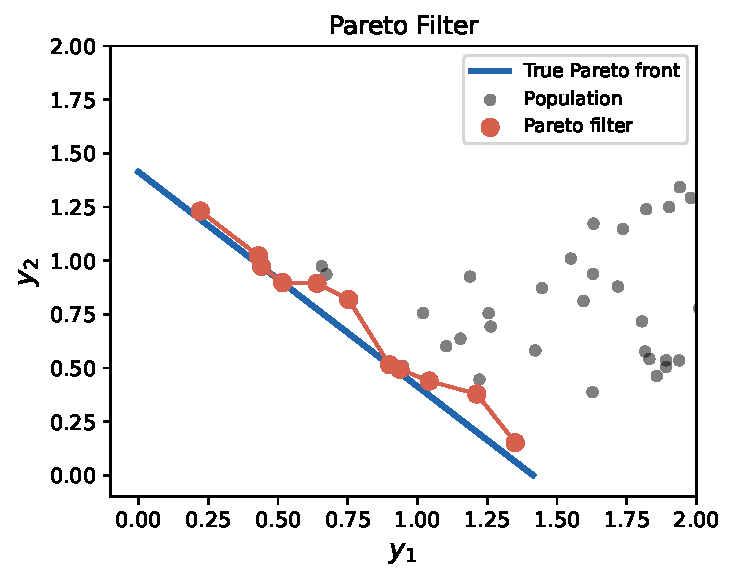
\includegraphics[width=\linewidth]{fig_pareto_filter.pdf}
\vspace{0.2em}
\small The filled red circles show the Pareto filter approximating the true
frontier (solid blue curve).  The filter is well-spread because closest-pair
pruning prevents clustering.
\end{columns}

\begin{alertblock}{Why Closest-Pair Pruning?}
  When the filter is over capacity, we must remove one point.  Removing the
  point with the \emph{worst} objective value is tempting but wrong: it would
  bias the archive toward the centre of the frontier and miss the extremes.
  Removing one of the \emph{closest pair} instead eliminates a redundant
  point (since the remaining one in the pair still represents that part of
  the frontier), while preserving the overall spread of the archive.
\end{alertblock}

\end{frame}

\begin{frame}[fragile]{Pareto Filter in Python}

\begin{lstlisting}
import numpy as np

def dominates(y, y_prime):
    return bool(np.all(y <= y_prime) and np.any(y < y_prime))

def discard_closest_pair(xs, ys):
    """
    Remove one point from the closest pair in criterion space.
    xs, ys : Python lists of design points and objective vectors.
    Modifies xs and ys in-place.
    """
    min_dist = np.inf
    pair_idx = (0, 1)
    for i in range(len(ys)):
        for j in range(i + 1, len(ys)):
            d = np.linalg.norm(ys[i] - ys[j])  # Euclidean distance
            if d < min_dist:
                min_dist = d
                pair_idx = (i, j)
    # Remove one of the closest pair at random
    idx_to_remove = np.random.choice(list(pair_idx))
    xs.pop(idx_to_remove)
    ys.pop(idx_to_remove)

def update_pareto_filter(filter_xs, filter_ys, xs, ys, capacity=None):
    """
    Add non-dominated points to the filter; prune if over capacity.
    filter_xs, filter_ys : current archive (modified in-place)
    xs, ys               : new candidate points to consider
    capacity             : maximum archive size (defaults to len(xs))
    """
    capacity = capacity or len(xs)
    # Step 1: Add new non-dominated points
    for x, y in zip(xs, ys):
        if not any(dominates(fy, y) for fy in filter_ys):
            filter_xs.append(x)
            filter_ys.append(y)
    # Step 2: Remove any dominated points from the updated filter
    fxs2, fys2 = [], []
    for x, y in zip(filter_xs, filter_ys):
        if not any(dominates(fy, y) for fy in filter_ys
                   if not np.array_equal(fy, y)):
            fxs2.append(x)
            fys2.append(y)
    filter_xs[:], filter_ys[:] = fxs2, fys2
    # Step 3: Prune if over capacity
    while len(filter_xs) > capacity:
        discard_closest_pair(filter_xs, filter_ys)
    return filter_xs, filter_ys
\end{lstlisting}

\end{frame}

\begin{frame}[allowframebreaks]{15.4.4 Niche Techniques}

Even with the methods above, population-based algorithms have a tendency to
\textbf{niching}: the population evolves toward a small cluster of similar
designs in one region of the Pareto frontier, failing to maintain diversity
across the full frontier.  This happens because individuals in a dense cluster
compete with each other, and crossover within a cluster generates more similar
offspring.

\textbf{Niche techniques} add deliberate mechanisms to spread the population
across the criterion space.

\begin{columns}
\column{0.55\textwidth}
\begin{block}{The Niching Problem}
  The population may converge to a few ``niches'' (dense clusters) in
  criterion space, failing to represent the full Pareto frontier.  This
  occurs because competitive selection favours \emph{locally} good individuals
  without rewarding \emph{global} diversity.
\end{block}

\begin{block}{Fitness Sharing}
  Penalise individuals by the number of other individuals in their
  neighbourhood in criterion space.  The modified (shared) fitness is:
  \[
    \tilde{f}_i(\bx) = f_i(\bx) \times
    \Bigl(1 + \alpha \cdot |\mathcal{N}_\sigma(\bx)|\Bigr)
  \]
  Here $\alpha$ (alpha) is the sharing strength (how heavily to penalise
  crowding), $\sigma$ (sigma) is the neighbourhood radius (how close two
  points must be to be considered neighbours), and
  $\mathcal{N}_\sigma(\bx) = \{\bx' : \|\bff(\bx') - \bff(\bx)\| < \sigma\}$
  (script N sub sigma of $x$) is the set of individuals within radius
  $\sigma$ of $\bx$ in criterion space.  The symbol $|\cdot|$ denotes the
  number of elements in the set.
\end{block}

\begin{alertblock}{How to Read the Fitness Sharing Formula}
  An individual in a densely populated region of criterion space has many
  neighbours ($|\mathcal{N}_\sigma|$ is large), so its fitness is multiplied
  by a large penalty factor.  This makes the selection algorithm less likely
  to choose it, even if it is otherwise good.  Individuals in sparsely
  populated regions have fewer neighbours and are penalised less, effectively
  rewarding diversity.
\end{alertblock}

\column{0.42\textwidth}
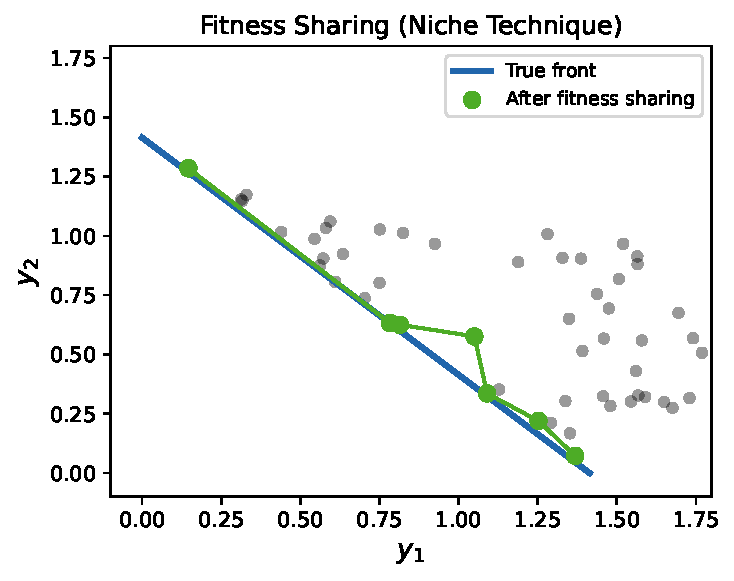
\includegraphics[width=\linewidth]{fig_fitness_sharing.pdf}
\small Fitness sharing spreads the population along the Pareto frontier,
dramatically improving coverage compared to basic selection.
\end{columns}

\begin{block}{Equivalence Class Sharing}
  An alternative to fitness sharing that is more directly integrated with
  nondomination ranking: when two individuals have the \emph{same}
  nondomination level, prefer the one with \emph{fewer nearby points} in
  criterion space.  This is essentially the crowding distance tiebreaker
  used in NSGA-II: among equally-ranked individuals, choose those that are
  more isolated, thereby spreading the population.
\end{block}

The key takeaway from Section 15.4 is that population methods, when combined
with nondomination ranking, elite archiving (Pareto filters), and
diversity-preserving mechanisms (niche techniques), can approximate the full
Pareto frontier in a single evolutionary run --- a major advantage over
scalarisation methods that require one run per frontier point.

\end{frame}

% =====================================================================
\section{Preference Elicitation}
% =====================================================================

\begin{frame}[allowframebreaks]{15.5 Preference Elicitation: Overview}

All the methods discussed so far either require the designer to specify
weights in advance (scalarisation) or produce the full Pareto frontier
(population methods).  But in practice, neither extreme is ideal:
specifying weights requires precise knowledge of one's preferences, and
the full frontier (which may contain thousands of points) gives no guidance
on which design to actually choose.

\textbf{Preference elicitation} takes a middle path.  Rather than asking the
designer to specify weights directly (which is cognitively difficult), it
presents a series of simple pairwise comparisons: ``Do you prefer design A or
design B?''  Each answer constrains which weight vectors are consistent with
the designer's preferences, gradually narrowing down the feasible weight set
until a clear winner emerges.

\begin{columns}
\column{0.55\textwidth}
\begin{block}{Goal of Preference Elicitation}
  Infer a scalar utility function from expert preferences about trade-offs,
  rather than asking the expert to specify weights numerically.  This is
  more natural because humans are generally better at comparing two specific
  options than at stating abstract numerical preferences.
\end{block}

\begin{block}{Underlying Model}
  We assume the designer's preferences are consistent with a
  \textbf{weighted-sum utility}: the designer prefers design $\ba$ to design
  $\bb$ if and only if $\bw^\top \ba < \bw^\top \bb$ for some (unknown)
  weight vector $\bw$.  Each expressed preference is then a linear constraint
  on $\bw$.  As we collect more preferences, the set $\mathcal{W}$ (script W,
  the set of consistent weight vectors, also called the \emph{weight polytope})
  shrinks.
\end{block}

\column{0.42\textwidth}
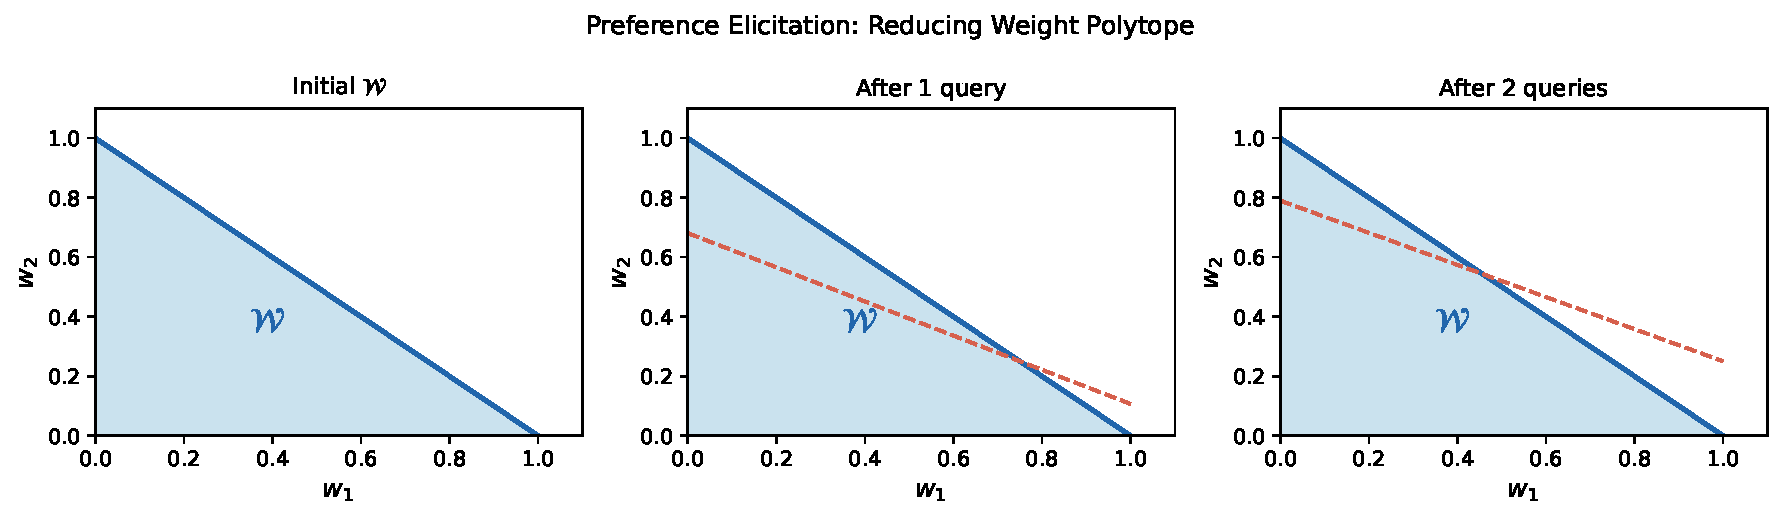
\includegraphics[width=\linewidth]{fig_preference_elicitation.pdf}
\small Each preference query adds a half-space constraint on $\bw$, cutting
the feasible weight polytope $\mathcal{W}$ in half (approximately).  After
enough queries, $\mathcal{W}$ is small enough to identify a clear best design.
\end{columns}

\begin{alertblock}{Key Insight}
  We never need to know the exact weight vector $\bw$.  We only need to know
  it well enough to confidently select one design over all others.  The
  stopping criterion (Section 15.5.3) formalises this: we stop asking
  questions when the \emph{minimax regret} falls below a threshold
  $\theta$ (theta).
\end{alertblock}

\end{frame}

\begin{frame}[allowframebreaks]{15.5.1 Model Identification}

This section formalises how pairwise preference queries constrain the
weight vector $\bw$.

\begin{columns}
\column{0.55\textwidth}
\begin{block}{Preference Constraints (Eq.\ 15.11--15.12)}
  Suppose the designer is shown $n$ pairs of designs
  $\{(\ba^{(i)}, \bb^{(i)})\}_{i=1}^n$ (the superscript $(i)$ in parentheses
  means ``the $i$-th pair'') and expresses that $\ba^{(i)}$ is preferred to
  $\bb^{(i)}$ in each case.  Under the weighted-sum model, this means:
  \[
    \bw^\top \ba^{(i)} < \bw^\top \bb^{(i)}
    \;\Longrightarrow\;
    \underbrace{(\ba^{(i)} - \bb^{(i)})^\top}_{\text{preference direction}} \bw < 0
  \]
  Each such preference defines a half-space in $\bw$-space: the vector
  $\bw$ must lie on the side where the above inequality holds.
\end{block}

A consistent weight vector satisfies all constraints simultaneously:
\[
  \begin{cases}
    (\ba^{(i)} - \bb^{(i)})^\top \bw < 0 & \forall\, i = 1, \ldots, n \\
    \mathbf{1}^\top \bw = 1
      & \text{(weights sum to one)} \\
    \bw \ge \mathbf{0}
      & \text{(no negative weights)}
  \end{cases}
\]
Here $\mathbf{1}$ (bold one) is the vector of all ones.  The symbol
$\forall$ (for all) means ``for every.''  The notation $\bw \ge \mathbf{0}$
means every component of $\bw$ is non-negative.

\begin{block}{Optimal $\bw$ (Eq.\ 15.13)}
  Among all weight vectors consistent with the expressed preferences, choose
  the one that \textbf{best separates} preferred designs from non-preferred
  ones:
  \[
    \min_{\bw}\; \sum_{i=1}^n (\ba^{(i)} - \bb^{(i)})^\top \bw
    \quad\text{subject to the constraints above}
  \]
  Alternatively, choose $\bw$ closest to the current estimate (stay close
  to what we know): $\min \|\bw - \bw^{(n)}\|_1$.
\end{block}

\column{0.42\textwidth}
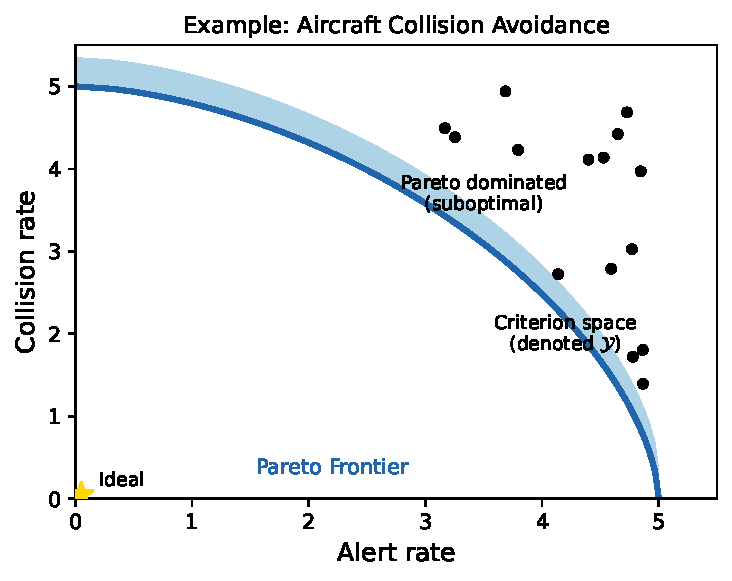
\includegraphics[width=\linewidth]{fig_collision_avoidance.pdf}
\small The collision-avoidance example: each preference query (``prefer lower
alert rate over lower collision rate'' or vice versa) adds a constraint on
$\bw$, narrowing $\mathcal{W}$.
\end{columns}

\end{frame}

\begin{frame}[fragile]{Preference Elicitation in Python}

The code below implements preference constraint satisfaction using linear
programming.  The function \texttt{update\_weights} takes the current weight
estimate and a list of preference pairs, and returns the updated weight vector
that best satisfies all constraints.

\begin{lstlisting}
import numpy as np
from scipy.optimize import linprog

def update_weights(prev_w, a_pts, b_pts):
    """
    Find weight vector w satisfying all preference constraints.
    Each pair (a_pts[i], b_pts[i]) means a_pts[i] is preferred over b_pts[i],
    i.e., w^T a_i < w^T b_i, i.e., (a_i - b_i)^T w < 0.

    prev_w : current weight estimate (m-vector)
    a_pts  : list of preferred design objective vectors
    b_pts  : list of non-preferred design objective vectors
    Returns: updated weight vector satisfying all constraints
    """
    n_pairs = len(a_pts)
    m = len(prev_w)
    eps = 1e-6  # strict inequality: (a-b)^T w <= -eps

    # Inequality constraints: (a_i - b_i)^T w <= -eps
    A_ub = np.array([a - b for a, b in zip(a_pts, b_pts)])
    b_ub = -eps * np.ones(n_pairs)

    # Equality constraint: sum(w) = 1
    A_eq = np.ones((1, m))
    b_eq = np.array([1.0])

    # Objective: minimize sum(w) (simple proxy; replace with L1 closeness)
    c = np.zeros(m)
    bounds = [(0, 1)] * m

    result = linprog(c, A_ub=A_ub, b_ub=b_ub,
                     A_eq=A_eq, b_eq=b_eq,
                     bounds=bounds, method='highs')
    return result.x if result.success else prev_w

# Example: 3 objectives, 1 preference
w0 = np.array([1/3, 1/3, 1/3])   # equal initial weights
a1 = np.array([0.2, 0.8, 0.6])   # preferred design (criterion vector)
b1 = np.array([0.9, 0.1, 0.2])   # non-preferred design
w_new = update_weights(w0, [a1], [b1])
print("Updated weights:", np.round(w_new, 3))
\end{lstlisting}

\end{frame}

\begin{frame}[allowframebreaks]{15.5.2 Paired Query Selection: Q-Eval}

The preference elicitation algorithm must decide \emph{which pair of designs}
to present to the designer at each step.  A naive approach (random pairs) is
inefficient: some queries provide almost no information about $\bw$ (e.g., if
we already know the designer would prefer one design overwhelmingly).
\textbf{Q-Eval} selects queries that maximally reduce uncertainty about $\bw$.

\begin{columns}
\column{0.55\textwidth}
\begin{block}{Q-Eval Algorithm}
  The goal is to select the query $(a, b)$ that cuts the feasible weight
  polytope $\mathcal{W}$ (script W) into two pieces of nearly equal volume.
  An equal split halves $|\mathcal{W}|$ in one query --- the most information
  possible.
  \begin{enumerate}
    \item Compute the \textbf{analytic center} $\mathbf{c}$ of $\mathcal{W}$:
    \[
      \mathbf{c} = \argmax_{\bw \in \mathcal{W}}
      \sum_{i=1}^n \ln\!\left[(\bb^{(i)} - \ba^{(i)})^\top \bw\right]
    \]
    The $\ln$ (natural logarithm) term pushes the center away from the
    boundary constraints; maximising the sum keeps $\mathbf{c}$ ``in the
    middle.''

    \item For each candidate design pair, compute the \emph{normal distance}
      from the bisecting hyperplane to $\mathbf{c}$.

    \item Sort pairs by distance; evaluate the $k$ closest candidates.

    \item Choose the pair with \textbf{volume ratio closest to $0.5$}
      (most equal split of $\mathcal{W}$).
  \end{enumerate}
\end{block}
\column{0.42\textwidth}
\begin{block}{Polyhedral Approximation Method}
  A computationally cheaper alternative: approximate $\mathcal{W}$ with a
  bounding \textbf{ellipsoid} (an $m$-dimensional generalised ellipse)
  centred at the analytic centre.  Select queries perpendicular to the
  \emph{longest axis} of the ellipsoid.  This axis represents the direction
  of greatest remaining uncertainty about $\bw$; cutting perpendicular to it
  reduces uncertainty fastest.  The ellipsoid shrinks and becomes more
  spherical as more queries are answered.
\end{block}

\begin{exampleblock}{Stopping Criterion: Minimax Regret (Eq.\ 15.16)}
  Stop asking queries when the \textbf{minimax regret} falls below a
  threshold $\theta$ (theta, a small positive number):
  \[
    x^* = \argmin_\bx \max_{\bw \in \mathcal{W}} \max_{\bx' \in \mathcal{X}}
    \bw^\top\!\bigl(\bff(\bx) - \bff(\bx')\bigr)
  \]
  Terminate when this minimax regret $< \theta$.
\end{exampleblock}
\end{columns}

\end{frame}

\begin{frame}[allowframebreaks]{15.5.3 Design Selection}

After collecting enough preference information to make $\mathcal{W}$ small,
we must select the \emph{final design} to recommend.  Two related methods
address this.

\begin{columns}
\column{0.55\textwidth}
\begin{block}{Decision Quality Improvement (Eq.\ 15.15)}
  Choose the design $x^*$ that minimises the \textbf{worst-case weighted
  objective} over all weight vectors in $\mathcal{W}$:
  \[
    x^* = \argmin_{\bx \in \mathcal{X}}\;
    \max_{\bw \in \mathcal{W}}\; \bw^\top \bff(\bx)
  \]
  Here $\max_{\bw \in \mathcal{W}}$ means ``consider the worst possible
  weight vector consistent with all observed preferences.''  The $\argmin$
  (arg min) returns the design $\bx$ that achieves the smallest value of
  this worst-case objective.  This gives an upper bound on the objective
  value: no matter which consistent $\bw$ turns out to be correct, the
  objective of $x^*$ cannot exceed this bound.
\end{block}

\begin{block}{Minimax Regret (Eq.\ 15.16)}
  The \textbf{regret} of choosing $\bx$ instead of $\bx'$ under weights $\bw$
  is the difference in their weighted objectives:
  \[
    \text{Regret}(\bx, \bx', \bw) =
    \bw^\top \bff(\bx) - \bw^\top \bff(\bx')
  \]
  The minimax regret criterion selects the design that minimises the maximum
  regret over all consistent weights and all alternative designs:
  \[
    x^* = \argmin_\bx\; \max_{\bw \in \mathcal{W}}\;
    \max_{\bx' \in \mathcal{X}}\; \text{Regret}(\bx, \bx', \bw)
  \]
\end{block}

\column{0.42\textwidth}
\begin{block}{Comparing the Two Criteria}
  \begin{itemize}
    \item \textbf{DQI} (Decision Quality Improvement) is \emph{conservative}:
      it guards against the worst possible set of weights, but may recommend
      an overly cautious design.

    \item \textbf{Minimax regret} is more nuanced: it asks not just ``is
      this design's objective small?'' but ``how much worse is this design
      than the best alternative, in the worst case?''  This accounts for the
      uncertainty in the utility model more directly.

    \item Both criteria are \textbf{robust} to errors in the weight
      estimates, since they optimise over the entire feasible set
      $\mathcal{W}$ rather than committing to a single point estimate.
  \end{itemize}
\end{block}

\begin{alertblock}{Key Use of Minimax Regret}
  Minimax regret serves a \textbf{dual purpose}: as a design selection
  criterion and as a \textbf{stopping criterion}.  Terminate the preference
  elicitation process (stop asking queries) when the minimax regret drops
  below a threshold $\theta$ (theta, chosen by the designer based on how
  much residual uncertainty is acceptable).
\end{alertblock}
\end{columns}

\begin{alertblock}{How to Read the Minimax Regret Formula}
  Think of regret as ``what you lost by choosing $\bx$ instead of the
  optimal $\bx'$.''  If you chose $\bx$ but the best design was actually
  $\bx'$, your regret is $\bw^\top\bff(\bx) - \bw^\top\bff(\bx') \ge 0$.
  Minimax regret minimises the worst case of this quantity: the designer
  is guaranteed that no matter which consistent weight vector $\bw$ is
  the true one, the chosen design $x^*$ will not perform more than
  $\theta$ worse than the best possible design.
\end{alertblock}

\end{frame}

% =====================================================================
\section{Summary \& Exercises}
% =====================================================================

\begin{frame}[allowframebreaks]{Chapter 15 Summary}

This chapter introduced the framework and main algorithms for
\textbf{multiobjective optimization}, where the goal is to minimise a
\emph{vector} of competing objective functions simultaneously.  The key
insight is that there is no single ``best'' solution: instead, there is a
set of Pareto-optimal designs, each representing a different trade-off.

\begin{columns}
\column{0.5\textwidth}
\begin{block}{Core Concepts}
  \textbf{Dominance} ($\bx$ dominates $\bx'$) means $\bx$ is at least as
  good on every objective and strictly better on at least one.  This partial
  ordering replaces the total ordering of single-objective optimisation.

  The \textbf{Pareto frontier} is the set of all non-dominated designs --- the
  boundary of the criterion space $\mathcal{Y}$.  Only frontier points are
  of interest to a rational designer.

  The \textbf{utopia point} gives the best achievable value for each objective
  independently, serving as an aspirational reference even though it is
  generally unattainable.
\end{block}

\begin{block}{Scalarisation Methods}
  The \textbf{constraint} ($\varepsilon$-constraint) method handles nonconvex
  frontiers by converting all but one objective into constraints.

  The \textbf{lexicographic} method optimises objectives in strict priority
  order, producing one Pareto-optimal point for a given priority ranking.

  The \textbf{weighted sum} method is the simplest but cannot find points in
  nonconvex frontier regions.

  The \textbf{weighted min-max (Tchebycheff)} method achieves complete
  coverage of any Pareto frontier by minimising the worst-case weighted
  deviation from the goal; the augmented version eliminates weakly
  Pareto-optimal points.
\end{block}

\column{0.47\textwidth}
\begin{block}{Population Methods}
  \textbf{VEGA} uses objective-specific subpopulations combined with
  cross-breeding, tending toward the extreme points of the frontier.

  \textbf{Nondomination ranking} (NSGA-II) assigns every individual a
  Pareto level and uses crowding distance to maintain diversity.  It is
  the most widely used multiobjective evolutionary algorithm.

  \textbf{Pareto filters} maintain an elite archive of non-dominated
  designs, updated incrementally with closest-pair pruning to control
  archive size and maintain spread.

  \textbf{Fitness sharing} and other niche techniques prevent the population
  from clustering in one region of the frontier.
\end{block}

\begin{block}{Preference Elicitation}
  Binary pairwise queries constrain the weight polytope $\mathcal{W}$,
  each query adding a half-space constraint.

  \textbf{Q-Eval} and the polyhedral method choose queries that maximally
  reduce $|\mathcal{W}|$, minimising the total number of queries needed.

  \textbf{Minimax regret} provides both a robust design selection criterion
  and a natural stopping condition for the elicitation process.
\end{block}
\end{columns}

\end{frame}

\begin{frame}[allowframebreaks]{Exercises: Key Problems}

\begin{block}{Exercise 15.1 --- Weighted Sum Limitation}
  \textbf{Question}: What is a disadvantage of the weighted sum method for
  computing the Pareto frontier?

  \textbf{Answer}: The weighted sum method cannot find Pareto-optimal points
  in \emph{nonconvex} (concave) regions of the Pareto frontier.  Geometrically,
  the iso-cost contours of the weighted sum are hyperplanes (straight lines in
  2D).  When the Pareto frontier bends inward (is concave), no hyperplane is
  tangent to it in that region, so the optimizer jumps from one convex portion
  of the frontier to another, skipping the concave portion entirely.  Methods
  with nonlinear iso-cost contours (Tchebycheff, constraint method) are needed
  to recover those points.
\end{block}

\begin{block}{Exercise 15.2 --- Why Population Methods?}
  \textbf{Question}: Why are population methods well-suited for multiobjective
  optimization?

  \textbf{Answer}: Non-population (single-solution) methods find only
  \emph{one} Pareto-optimal point per run.  To approximate the full frontier
  with $k$ points, they require $k$ separate optimisation runs with different
  parameters (different weights or constraint levels).  Population methods,
  by contrast, maintain a \emph{collection} of designs that evolves together.
  Through mechanisms like nondomination ranking and fitness sharing, a single
  run naturally produces a diverse, well-spread collection of Pareto-optimal
  points spanning the entire frontier.
\end{block}

\begin{block}{Exercise 15.3 --- Dominance Example}
  \textbf{Question}: Consider the four criterion points
  $\{[1,2],\; [2,1],\; [2,2],\; [1,1]\}$.  Which are Pareto-optimal?

  \textbf{Answer}: $[1,1]$ dominates all others: $1 \le 2$, $1 \le 1$
  (for $[2,1]$: $1 < 2$ on $f_1$, $1 = 1$ on $f_2$, so yes it dominates).
  Actually, $[1,2]$ and $[2,1]$ are weakly Pareto-optimal because no other
  point is strictly better on \emph{both} objectives simultaneously.
  Only $[1,1]$ is a strictly Pareto-optimal point (it dominates $[1,2]$,
  $[2,1]$, and $[2,2]$).  The point $[2,2]$ is dominated by $[1,1]$
  (since $1 \le 2$ on both objectives and $1 < 2$ on both).
\end{block}

\end{frame}

\begin{frame}[allowframebreaks]{Exercise 15.7: Constraint Method Pareto Curve}

\begin{columns}
\column{0.52\textwidth}
\begin{block}{Problem Statement}
  Minimize $[f_1(x),\; f_2(x)] = [x^2,\; (x-2)^2]$ over all $x \in \mathbb{R}$.
  Use the constraint method to derive the Pareto curve analytically.
\end{block}

\begin{block}{Solution}
  We fix $f_2(x) = (x-2)^2 \le c$ (where $c \ge 0$ is the constraint bound)
  and minimise $f_1(x) = x^2$.

  The constraint $f_2(x) \le c$ means $(x-2)^2 \le c$, which is equivalent
  to $2 - \sqrt{c} \le x \le 2 + \sqrt{c}$.

  To minimise $f_1(x) = x^2$ over this interval:
  \[
    x^* =
    \begin{cases}
      2 - \sqrt{c} & \text{if } 2 - \sqrt{c} > 0,\; \text{i.e., } c < 4 \\
      0            & \text{if } 0 \in [2-\sqrt{c},\; 2+\sqrt{c}],
                     \text{ i.e., } c \ge 4 \\
      \text{infeasible} & \text{if } c < 0
    \end{cases}
  \]
  For $c \in [0, 4)$: $x^* = 2 - \sqrt{c}$.  The Pareto curve is then
  parametrised by $c \in [0, 4]$:
  \begin{align*}
    y_1 &= f_1(x^*) = (2 - \sqrt{c})^2 \\
    y_2 &= f_2(x^*) = (x^* - 2)^2 = (\,-\sqrt{c}\,)^2 = c
  \end{align*}
  The curve runs from $(y_1, y_2) = (4, 0)$ at $c=0$ to $(0, 4)$ at $c=4$.
\end{block}

\column{0.45\textwidth}
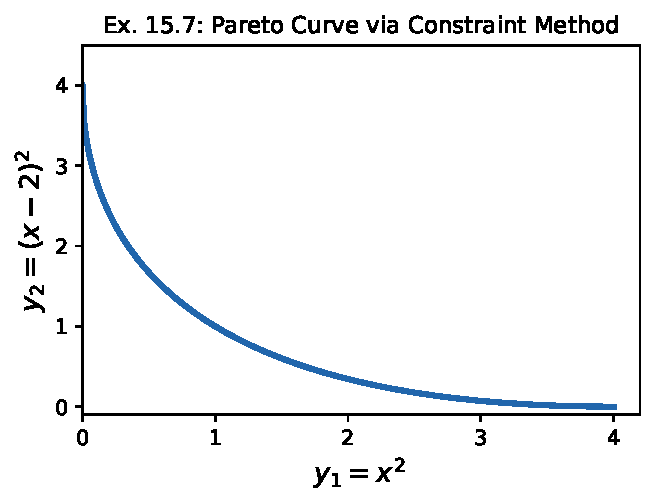
\includegraphics[width=\linewidth]{fig_exercise_pareto_curve.pdf}
\vspace{0.2em}
\small The Pareto curve for $[x^2,\; (x-2)^2]$ is the arc connecting
$(4, 0)$ to $(0, 4)$.  Every point on this arc is Pareto-optimal: reducing
$y_1$ necessarily increases $y_2$ and vice versa.
\end{columns}

\begin{exampleblock}{Numerical Check at Three Points}
  \begin{center}
  \begin{tabular}{lcccc}
  \toprule
  $c$ & $\sqrt{c}$ & $x^* = 2 - \sqrt{c}$ & $y_1 = (x^*)^2$ & $y_2 = c$ \\
  \midrule
  0   & 0    & 2       & 4    & 0 \\
  1   & 1    & 1       & 1    & 1 \\
  4   & 2    & 0       & 0    & 4 \\
  \bottomrule
  \end{tabular}
  \end{center}
  At $c = 1$: $x^* = 1$, so $f_1 = 1^2 = 1$ and $f_2 = (1-2)^2 = 1$.
  This is the symmetric midpoint of the Pareto curve.  Note that as $c$
  increases from 0 to 4, $y_1$ \emph{decreases} from 4 to 0 while $y_2$
  \emph{increases} from 0 to 4 --- the fundamental trade-off.
\end{exampleblock}

\end{frame}

\begin{frame}[allowframebreaks]{Exercise 15.3 Visualisation}

\begin{columns}
\column{0.5\textwidth}
\begin{block}{Example: 4 Criterion Points}
  Consider the four criterion points:
  $[1,2]$, $[2,1]$, $[2,2]$, $[1,1]$.

  \textbf{$[1,1]$}: This point dominates all three others.  It achieves
  $f_1 = 1 \le 2$ and $f_2 = 1 \le 2$ compared to $[2,2]$ (dominated),
  $f_1 = 1 \le 1$ and $f_2 = 1 < 2$ compared to $[1,2]$ (dominated),
  and $f_1 = 1 < 2$ and $f_2 = 1 \le 1$ compared to $[2,1]$ (dominated).
  So $[1,1]$ is strictly Pareto-optimal.

  \textbf{$[1,2]$}: Dominated by $[1,1]$ ($f_1$ ties, $f_2$ is worse).
  However, no other point strictly beats $[1,2]$ on both objectives
  simultaneously (it achieves $f_1 = 1$ which ties the best), so it is
  weakly Pareto-optimal.

  \textbf{$[2,1]$}: Similarly, dominated by $[1,1]$, but weakly Pareto-optimal.

  \textbf{$[2,2]$}: Strictly dominated by $[1,1]$ (worse on both objectives).
  Not Pareto-optimal in any sense.
\end{block}
\column{0.47\textwidth}
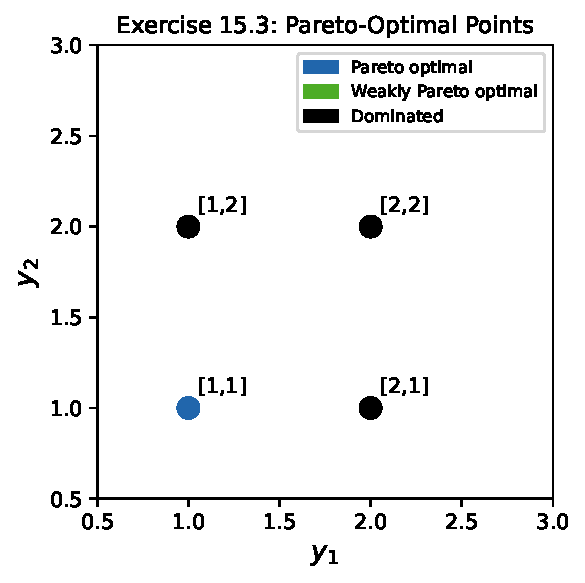
\includegraphics[width=\linewidth]{fig_exercise_example.pdf}
\end{columns}

\end{frame}

\begin{frame}[allowframebreaks]{Chapter 15: Key Takeaways}

\begin{enumerate}
  \item \textbf{Dominance is the fundamental partial ordering} for
    multiobjective problems.  It replaces the total order ($\le$) of
    single-objective optimisation.  Design $\bx$ dominates $\bx'$ if and
    only if it is at least as good on every objective and strictly better
    on at least one.

  \item \textbf{The Pareto frontier --- not a single point --- is the
    solution} to a multiobjective problem.  Every non-frontier point is
    provably suboptimal and can be discarded.

  \item \textbf{Scalarisation methods} reduce the multiobjective problem to
    a sequence of single-objective problems.  The \emph{augmented Tchebycheff}
    (weighted min-max) method is the most general, achieving complete coverage
    of any Pareto frontier including nonconvex portions.

  \item \textbf{Population methods} naturally spread across the Pareto
    frontier in a single run.  \textbf{NSGA-II} (nondomination ranking plus
    crowding distance) is the most widely used multiobjective evolutionary
    algorithm and is the recommended starting point for practical applications.

  \item \textbf{Preference elicitation} allows the designer to specify
    preferences implicitly (through pairwise comparisons) rather than
    explicitly (through numerical weights).  Each comparison adds a linear
    constraint on the weight polytope $\mathcal{W}$.

  \item \textbf{Minimax regret} provides a principled, robust criterion for
    both selecting the final design and deciding when to stop eliciting
    preferences.  It guarantees that the chosen design is never more than
    $\theta$ worse than the theoretically best design, regardless of which
    consistent weight vector is the truth.
\end{enumerate}

\begin{block}{Next Chapter}
  \textbf{Chapter 16: Sampling Plans} addresses a different but related
  challenge: how to efficiently explore the design space when function
  evaluations are expensive.  Topics include space-filling designs,
  Latin hypercube sampling (LHS), and quasi-random sequences.
\end{block}

\end{frame}

\end{document}
